\documentclass[17pt,a4paper]{extarticle}

% 1 inch margins
\usepackage[margin=1in]{geometry}
\usepackage{tcolorbox}
\usepackage{amsmath}
\usepackage{graphicx}
\usepackage{subcaption}
\usepackage{listings}
\usepackage{float}


% Line spacing (optional)
\usepackage{setspace}
\onehalfspacing % remove if not needed

\newtcolorbox{conceptbox}[1]{title=#1, fontupper=\small}
\lstset{
    language=Python,
    basicstyle=\ttfamily\small,
    keywordstyle=\bfseries,
    stringstyle=\ttfamily,
    showstringspaces=false,
    breaklines=true,
    frame=single,
}


\begin{document}

\section*{CHSH Inequality}
\subsection*{Motivation for the CHSH Inequality}
Bell’s original inequality showed that the predictions of quantum mechanics cannot be explained by classical theories based on predetermined measurement results. However, the original form of Bell’s inequality was difficult to test in real experiments because it assumed ideal conditions(Perfect detectors, No background interference, No experimental loopholes etc.) and perfect correlations(If observer $A$ measures “up”, Observer $B$ measures “down” with 100\% certainty).

To solve this problem, \textbf{John Clauser}, \textbf{Michael Horne}, \textbf{Abner Shimony}, and \textbf{Richard Holt} reformulated Bell’s inequality in 1969. Their work led to the CHSH inequality, which was designed specifically to be tested using real experimental setups. The CHSH form works with measurements that have only two possible outcomes, making it suitable for experiments with photons, electrons, and other quantum particles.

\begin{conceptbox}{Measurement in Quantum Mechanics}
\textit{Measurement in quantum mechanics is the act of interacting with a quantum system to obtain a definite outcome, causing the system to change from a superposition of states to a single observable result. But in classical physics objects already have definite properties, observation only reveals what was already there. In Bell and CHSH experiments, measuring a property like spin or polarization gives a binary result($\pm1$)}
\end{conceptbox}

The CHSH inequality provides a clear way to combine measurement results from two distant observers into a single quantity that can be compared with theoretical predictions. So we can test whether experimental results follow classical expectations or quantum mechanical predictions.

The CHSH inequality is also easy to implement in computer simulations. The mathematical form of the inequality allows correlations to be calculated using simple programs. Today, the CHSH inequality is widely used in quantum research to test entanglement and to support the development of quantum technologies such as quantum computing and secure quantum communication.

\subsection*{CHSH Experimental Setup}
The CHSH inequality considers an experiment involving two distant observers, called Alice and Bob, who share a pair of entangled particles. These particles are part of a single quantum state and they are separated so that one particle travels to Alice and the other to Bob. Each observer can choose two different measurement settings, which are labeled as $A$ and $A'$ for Alice, and $B$ and $B'$ for Bob.

\begin{conceptbox}{What is a Measurement Setting?}
\textit{A measurement setting is the choice of how you measure a quantum system. It means which direction, angle or basis you choose before performing the measurement. The setting choosen is completely upto the experimenter. For example, ``Alice sets her polarizer at 0$^\circ$''. This fixes how the photon is measured. This angle 0$^\circ$ is one measurement setting.}
\end{conceptbox}

When a measurement is performed, each observer records one of two possible outcomes, represented as $+1$ or $-1$. The choice of measurement setting is made independently by Alice and Bob, and the measurements are repeated many times to collect statistical data. The purpose of using two measurement setting for each observer is to study how different combinations of settings affect the correlations between the measurement outcomes.

This experimental setup is ready for real laboratory tests like photon polarization and electron spin measurement experiments. It is also easy to reproduce in computer simulations.

\subsection*{Correlation Functions}
In CHSH experiments, the result of a single measurement is not the important part. The relationship between the results obtained by Alice and Bob is the important part. This relationship is described using a correlation function, written as $E(A,B)$.

To calculate a correlation function, the experiment is repeated many times using the same pair of measurement settings. Everytime Alice and Bob record outcomes of either +1 or -1. The correlation is then obtained by averaging the product of their outcomes.
\begin{itemize}
    \item If the outcomes match $\rightarrow +ve$ correlation
    \item If the outcomes are opposite $\rightarrow -ve$ correlation
    \item If no pattern $\rightarrow 0$ correlation
\end{itemize}
By calculating correlation functions for different combinations of measurement settings, it is possible to construct the CHSH parameter and compare experimental or simulated results with classical and quantum predictions. Since correlation functions depend only on statistical data, they are easy to compute in both laboratory experiments and computer simulations.

\subsection*{Mathematical Form of the CHSH Inequality}
The CHSH inequality combines several correlation functions into a single quantity called the CHSH parameter, denoted by $S$. This parameter is defined using four different combinations of measurement settings chosen by Alice and Bob. Mathematically, it is written as
\begin{equation*}
S=E(A,B)+E(A,B')+E(A',B)-E(A',B')
\end{equation*}
where each term represents a correlation function for a specific pair of measurement settings.

The value of $S$ is calculated using experimental or simulated data. When the system follows classical expectations, the absolute value of $S$ is always less than or equal to $2$. This limit is known as the \textbf{classical} or \textbf{Bell bound}.

This simple mathematical form of CHSH inequality is useful because once we know the correlation functions, CHSH parameter can be easily calculated using numerical formula. Also classical and quantum predictions can be directly compared using the same mathematical form.

\subsection*{Classical Predictions and Numerical Simulation}
According to classical physics, the outcomes of measurements are assumed to be pre-determined the properties of the particles. When this is applied to the CHSH setup, the correlations between measurement outcomes are limited. As a result, the value of the CHSH parameter $S$ calculated always satisfies the inequality $|S|\leq2$.

In a classical numerical simulation, this behavior can be reproduced by assigning predefined values to each measurement setting and then calculating the resulting correlations. By repeating this process many times and averaging the results, the correlation functions and the CHSH parameter can be obtained. No matter how the predefined values are chosen, the final value of $S$ never exceeds the classical limit of $2$.

\subsubsection*{Classical Experiment}
Alice and Bob are standing some distance far away from one another. And there is another person named Victor between them. Victor prepares particle pairs with predefined values and sends those to Alice and Bob. Alice and Bob get same number of particles. Alice and Bob measures either $X$ or $Y$ projection of the particle they got.

\begin{figure}[h]
    \centering
    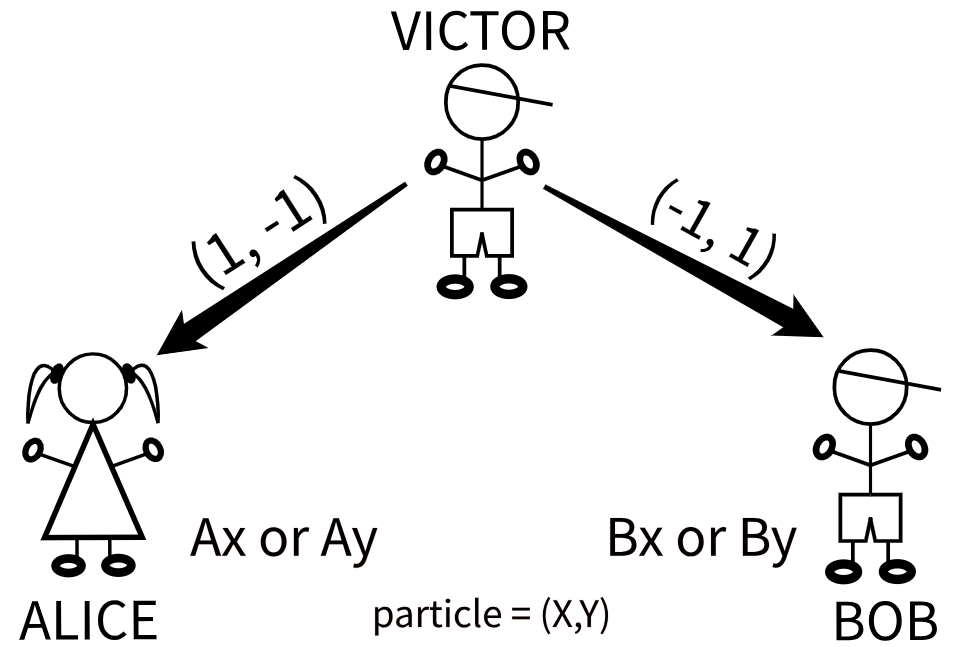
\includegraphics[width=0.5\textwidth]{images/bobandalice.png}
\end{figure}

$A_X$ and $A_Y$ are the $X$ and $Y$ projections of a particle measured by Alice, likewise $B_X$ and $B_Y$ by Bob. Every measurement has the value $\pm1$. The CHSH parameter is given by
\begin{equation}
S=A_XB_X+A_XB_Y+A_YB_X-A_YB_Y
\end{equation}
\begin{equation}
S=(A_X+A_Y)B_X+(A_X-A_Y)B_Y
\end{equation}

For any values of $A_X$ and $A_Y$, either $(A_X+A_Y)$ or $(A_X-A_Y)$ is zero. This means either $(A_X+A_Y)B_X$ or $(A_X-A_Y)B_Y$ has the value $\pm2$.

\begin{equation}
|S|=2
\end{equation}

We repeat the experiment many times and compute average value of each correlation function. From these averaged correlations, the following CHSH parameter is obtained.
\setcounter{equation}{0}
\begin{equation}
S=\langle A_XB_X \rangle+\langle A_XB_Y \rangle+\langle A_YB_X\rangle -\langle A_YB_Y \rangle
\end{equation}
Now the absolute value of $S$ bounded by 2.
\begin{equation}
|S|\leq2
\end{equation}
\subsubsection*{Python Simulation}
\begin{enumerate}
    \item Import Numpy and Matplotlib.
    \begin{lstlisting}
import numpy as np
import matplotlib.pyplot as plt
    \end{lstlisting}
    \item Initialise empty lists for $|S|$ and Trial number.
    \begin{lstlisting}
trials = []
S_abs_values = []
    \end{lstlisting}
    \item Input no of particle pairs($N$) and define correlation function(Average of product).
    \begin{lstlisting}
N = int(input("No of particle pairs: "))

def correlation(a, b):
    return np.mean(a * b)
    \end{lstlisting}
    \item Print table headings. Start a \textit{for} loop for desired no of trials(eg. 100). For every run, Alice measures $A_X$ and $A_Y$ of particle she got and Bob measures $B_X$ and $B_Y$ for particle he got. Even though they can only measure either X or Y at a time, we take both data because we need correlation between all measurement setting. Calcualte all four correlations using correlation function. Calcualte CHSH parameter. Append trial no. and $|S|$ to their lists. Print values of all correlations, $S$ and $|S|$.
    \begin{lstlisting}
print("E_xx\tE_xy\tE_yx\tE_yy\tS\t|S|")

for i in range(100):

    alice_X = np.random.choice([1, -1], N)
    alice_Y = np.random.choice([1, -1], N)

    bob_X   = np.random.choice([1, -1], N)
    bob_Y   = np.random.choice([1, -1], N)

    E_xx = correlation(alice_X, bob_X)
    E_xy = correlation(alice_X, bob_Y)
    E_yx = correlation(alice_Y, bob_X)
    E_yy = correlation(alice_Y, bob_Y)

    S = E_xx + E_xy + E_yx - E_yy

    trials.append(i)
    S_abs_values.append(abs(S))

    print(f"{E_xx:7.4f}\t{E_xy:7.4f}\t{E_yx:7.4f}\t{E_yy:7.4f}\t{S:7.4f}\t{abs(S):.4f}")
    \end{lstlisting}
    \item Plot trial no. in x-axis and $|S|$ in y-axis. Lable both axes. Enable grid. Apply limit(0-2) in y-axis. Give title for the plot. Save obtained graph in PNG format.
    \begin{lstlisting}
plt.plot(trials, S_abs_values, ".")
plt.xlabel("Trial number")
plt.ylabel("|S|")
plt.grid(axis="y")
plt.ylim(0, 2)
plt.title(f"Classical CHSH Simulation (N = {N})")
plt.savefig(f"Classical_CHSH_N_{N}.png", dpi=300, bbox_inches="tight")
plt.close()
    \end{lstlisting}
\end{enumerate}

\begin{lstlisting}[language=Python, basicstyle=\ttfamily\footnotesize]
import numpy as np
import matplotlib.pyplot as plt

trials = []
S_abs_values = []

N = int(input("No of particle pairs: "))

def correlation(a, b):
    return np.mean(a * b)

print("E_xx\tE_xy\tE_yx\tE_yy\tS\t|S|")

for i in range(100):

    alice_X = np.random.choice([1, -1], N)
    alice_Y = np.random.choice([1, -1], N)

    bob_X   = np.random.choice([1, -1], N)
    bob_Y   = np.random.choice([1, -1], N)

    E_xx = correlation(alice_X, bob_X)
    E_xy = correlation(alice_X, bob_Y)
    E_yx = correlation(alice_Y, bob_X)
    E_yy = correlation(alice_Y, bob_Y)

    S = E_xx + E_xy + E_yx - E_yy

    trials.append(i)
    S_abs_values.append(abs(S))

    print(f"{E_xx:7.4f}\t{E_xy:7.4f}\t{E_yx:7.4f}\t{E_yy:7.4f}\t{S:7.4f}\t{abs(S):.4f}")

plt.plot(trials, S_abs_values, ".")

plt.xlabel("Trial number")
plt.ylabel("|S|")
plt.grid(axis="y")
plt.ylim(0, 2)

plt.title(f"Classical CHSH Simulation (N = {N})")

plt.savefig(f"Classical_CHSH_N_{N}.png", dpi=300, bbox_inches="tight")
plt.close()
\end{lstlisting}
\newpage
\subsubsection*{Obtained Graphs}
\begin{figure}[h!]
\centering

% ---- Row 1 ----
\begin{subfigure}{0.44\textwidth}
    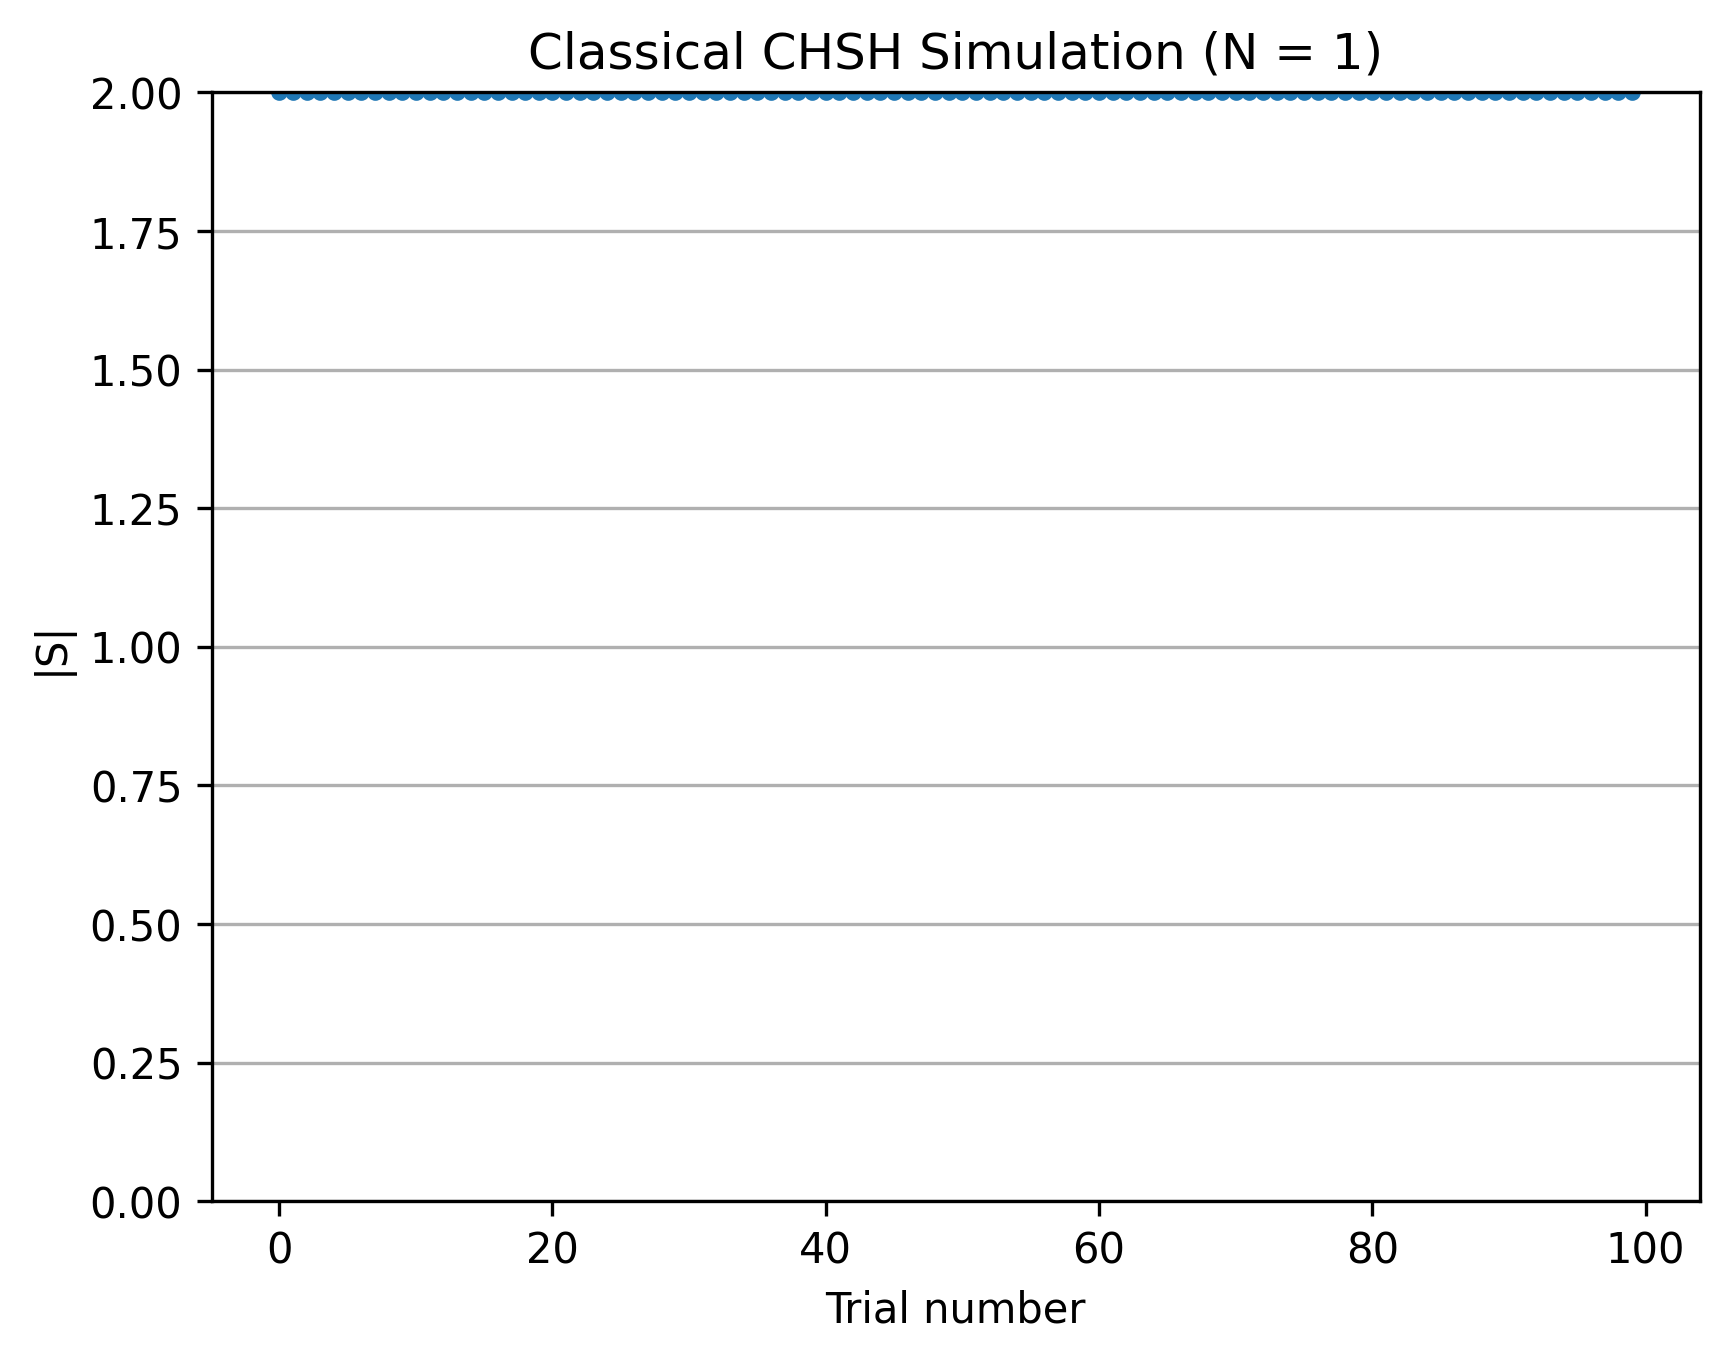
\includegraphics[width=\linewidth]{images/classical_sims/Classical_CHSH_N_1.png}
\end{subfigure}
\hfill
\begin{subfigure}{0.44\textwidth}
    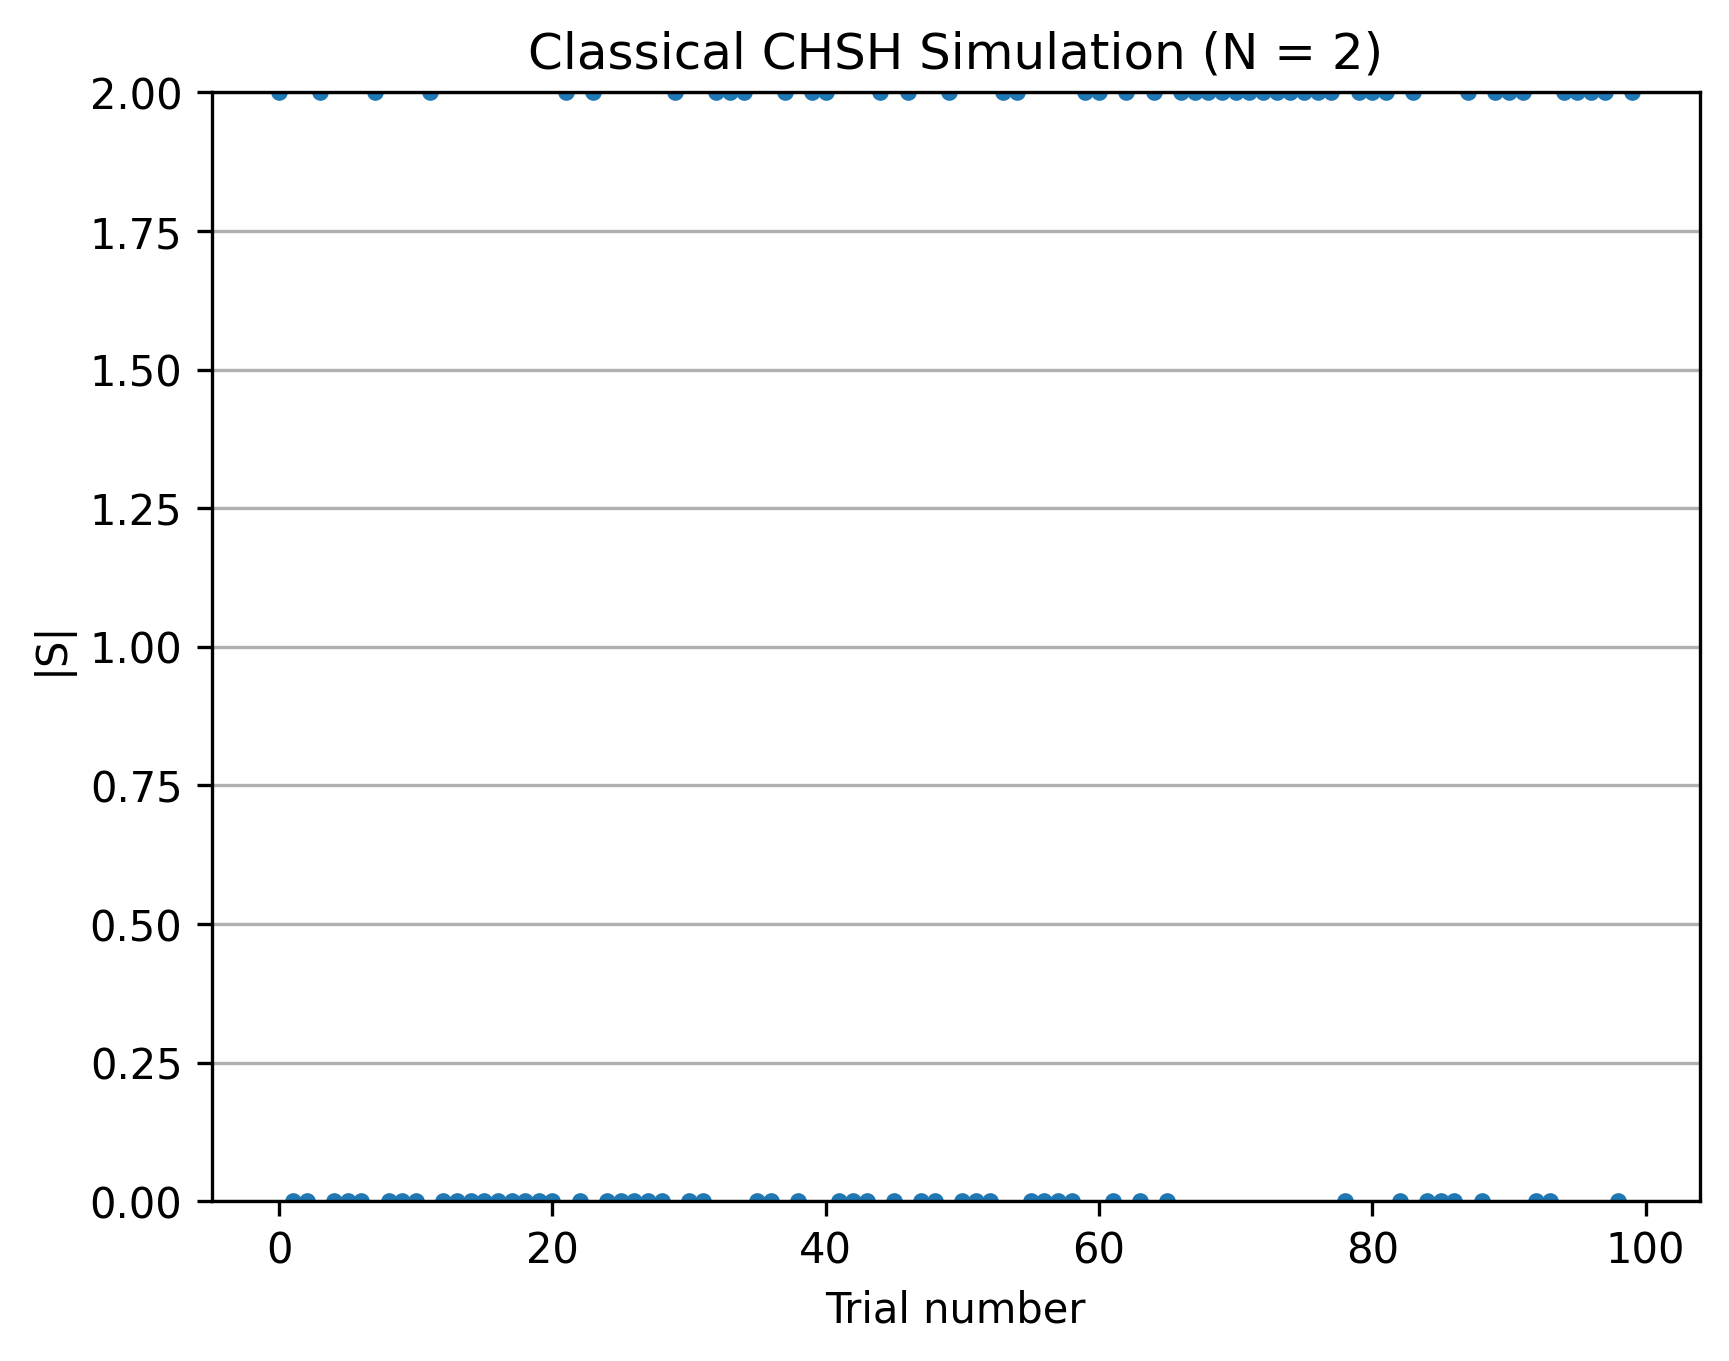
\includegraphics[width=\linewidth]{images/classical_sims/Classical_CHSH_N_2.png}
\end{subfigure}

\vspace{0.1cm}

% ---- Row 2 ----
\begin{subfigure}{0.44\textwidth}
    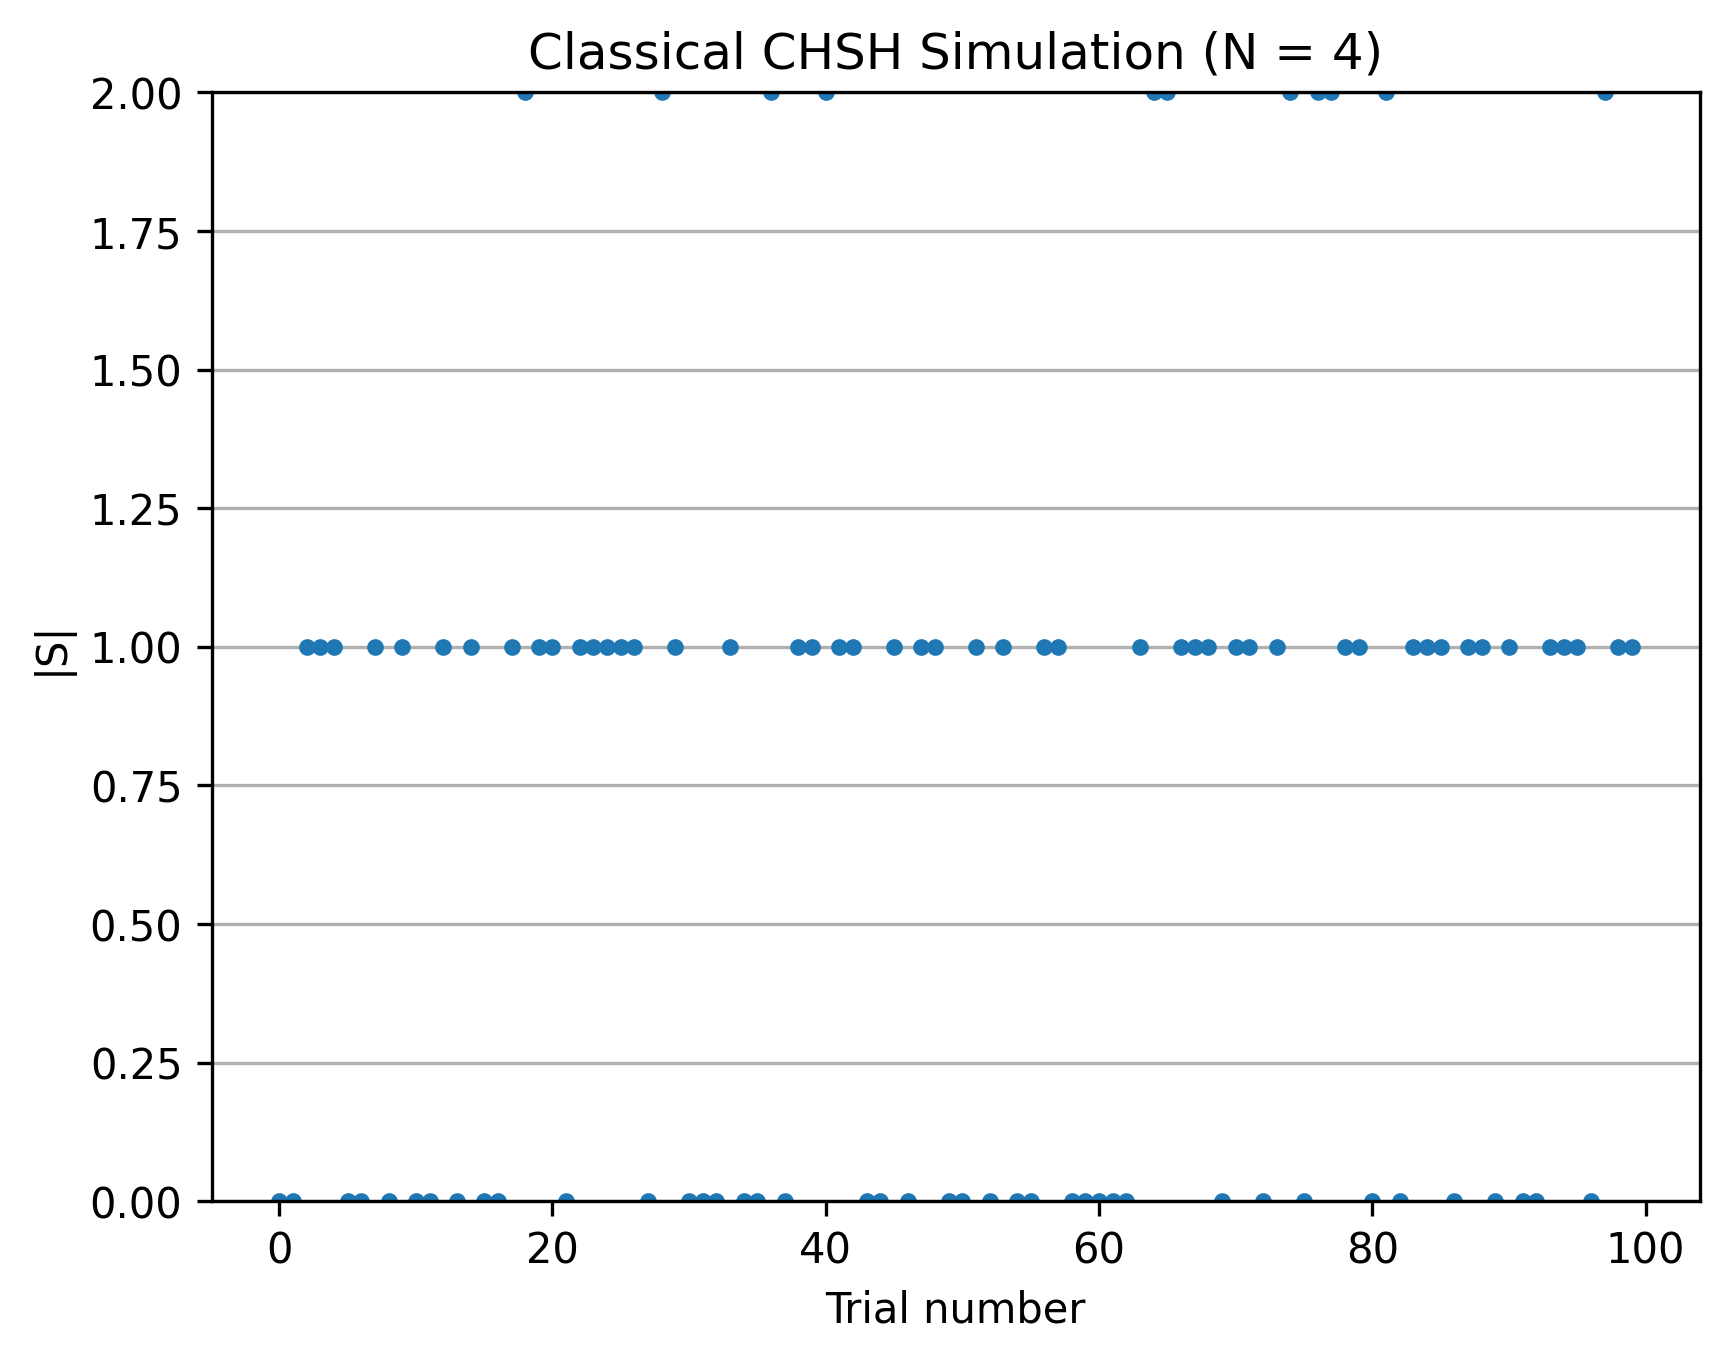
\includegraphics[width=\linewidth]{images/classical_sims/Classical_CHSH_N_4.png}
\end{subfigure}
\hfill
\begin{subfigure}{0.44\textwidth}
    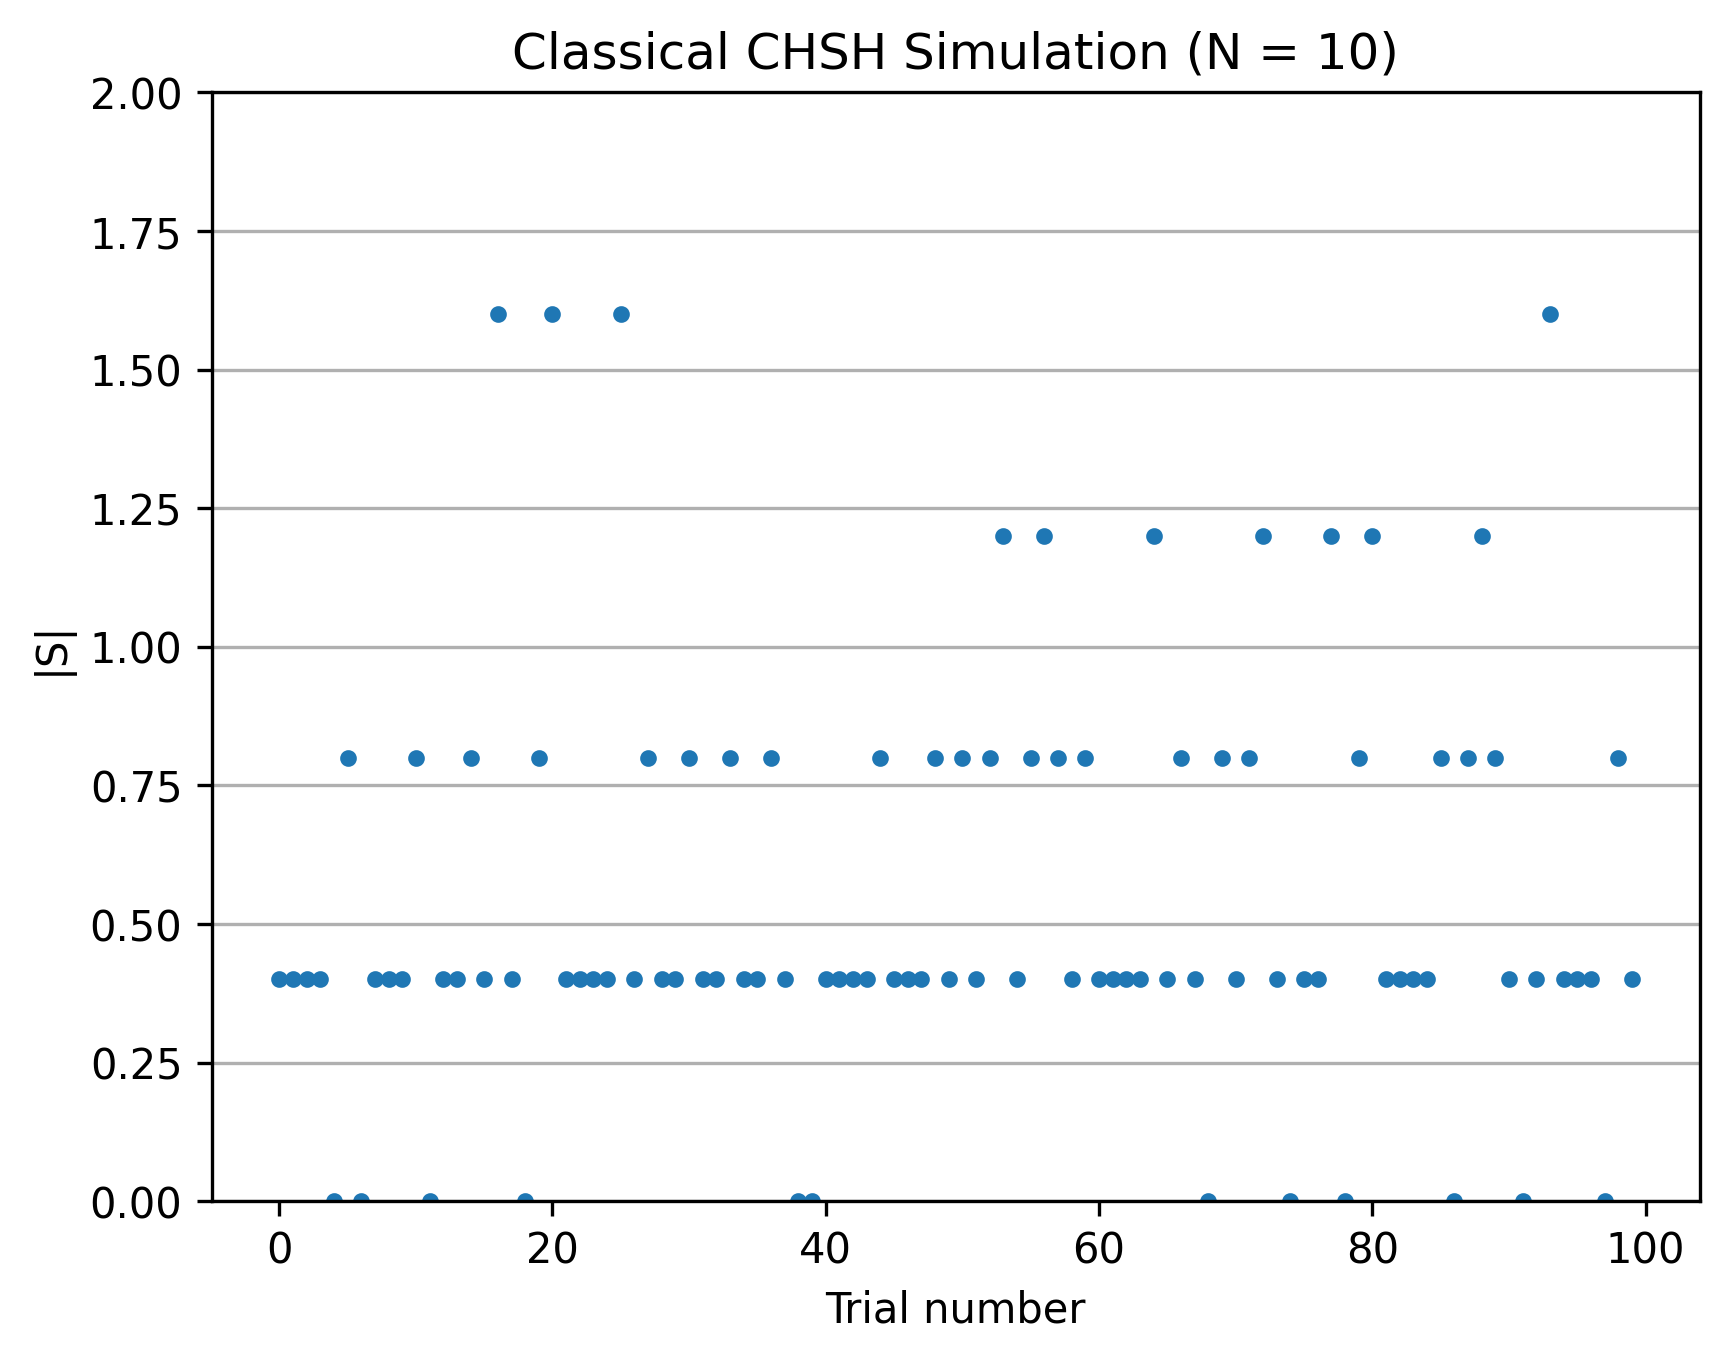
\includegraphics[width=\linewidth]{images/classical_sims/Classical_CHSH_N_10.png}
\end{subfigure}

\vspace{0.1cm}

% ---- Row 3 ----
\begin{subfigure}{0.44\textwidth}
    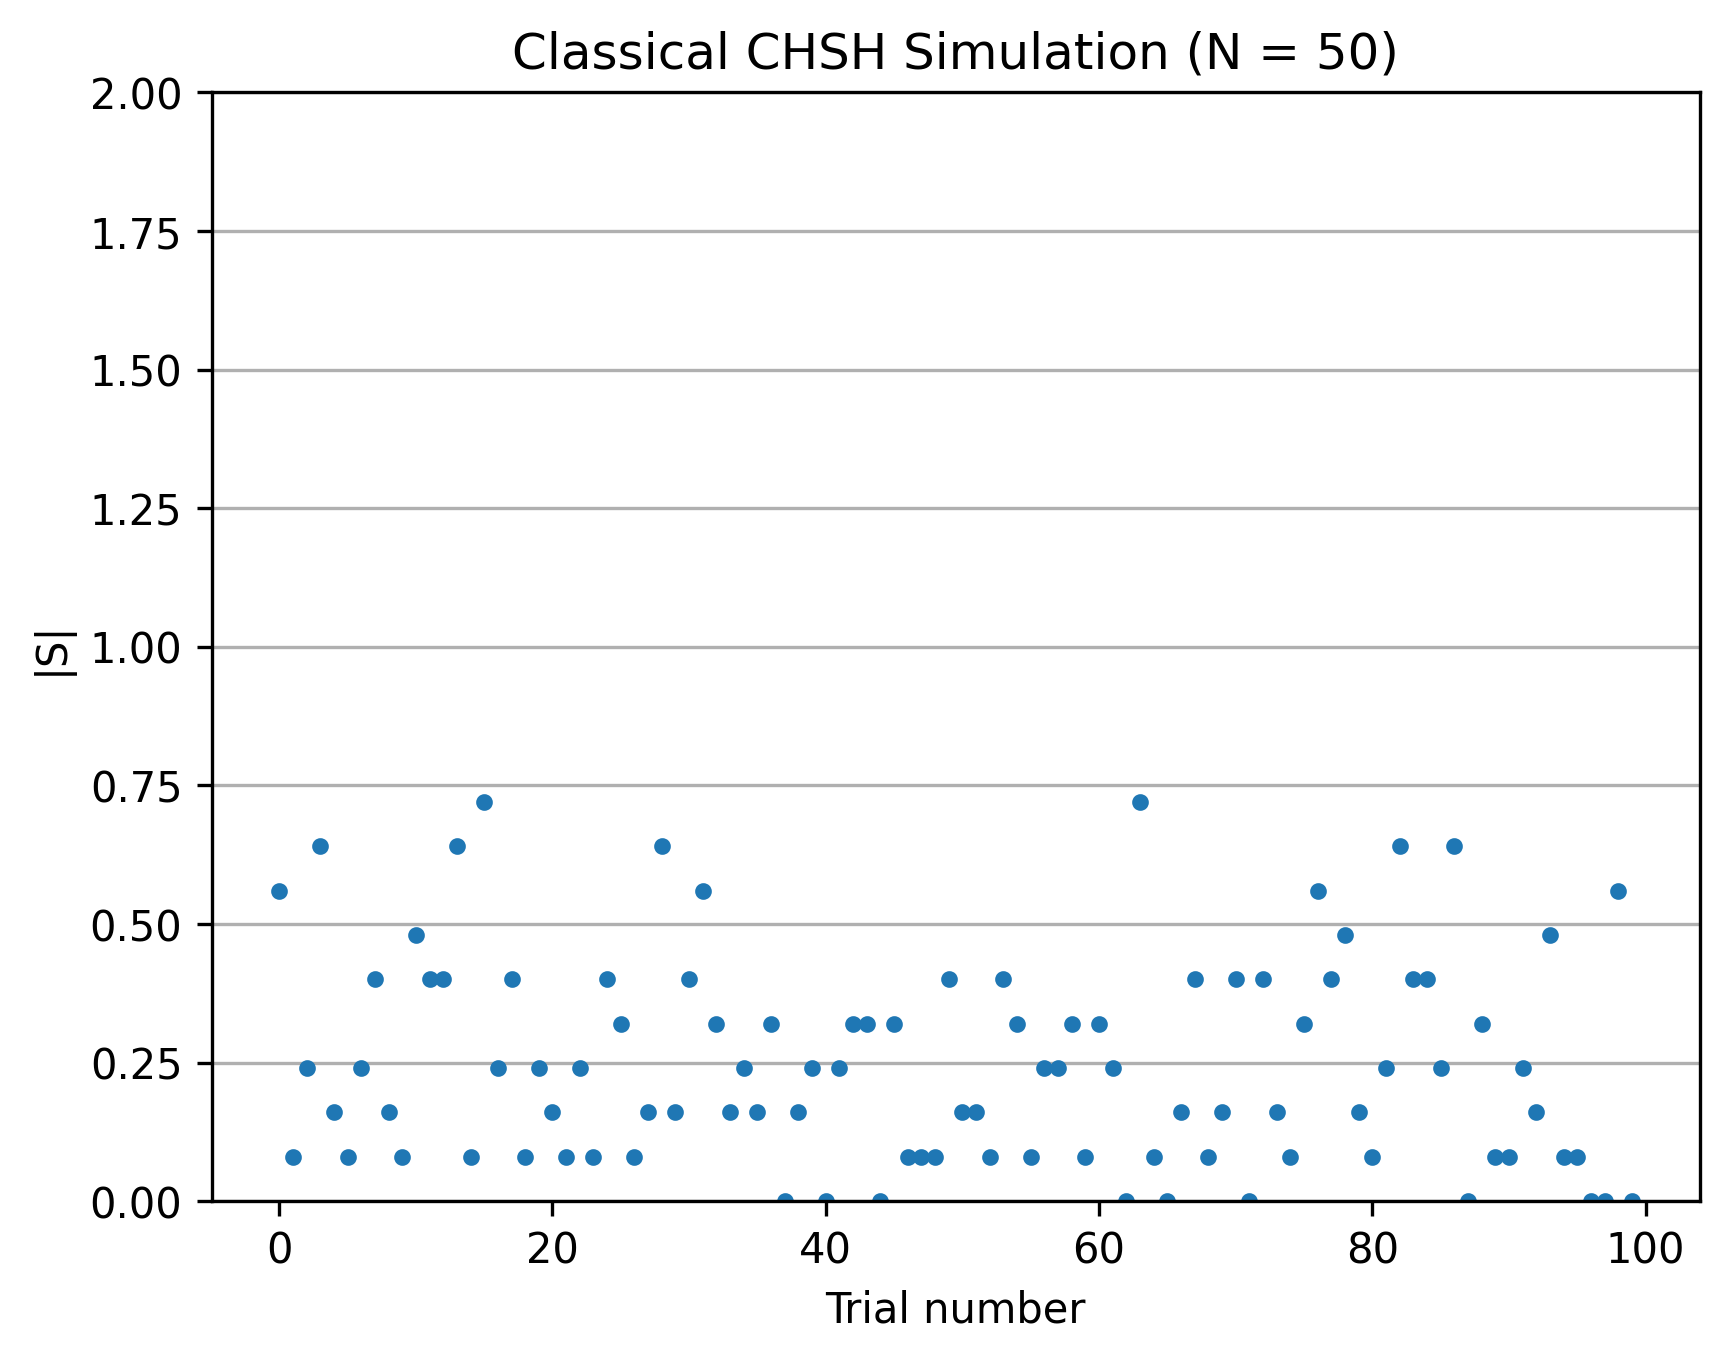
\includegraphics[width=\linewidth]{images/classical_sims/Classical_CHSH_N_50.png}
\end{subfigure}
\hfill
\begin{subfigure}{0.44\textwidth}
    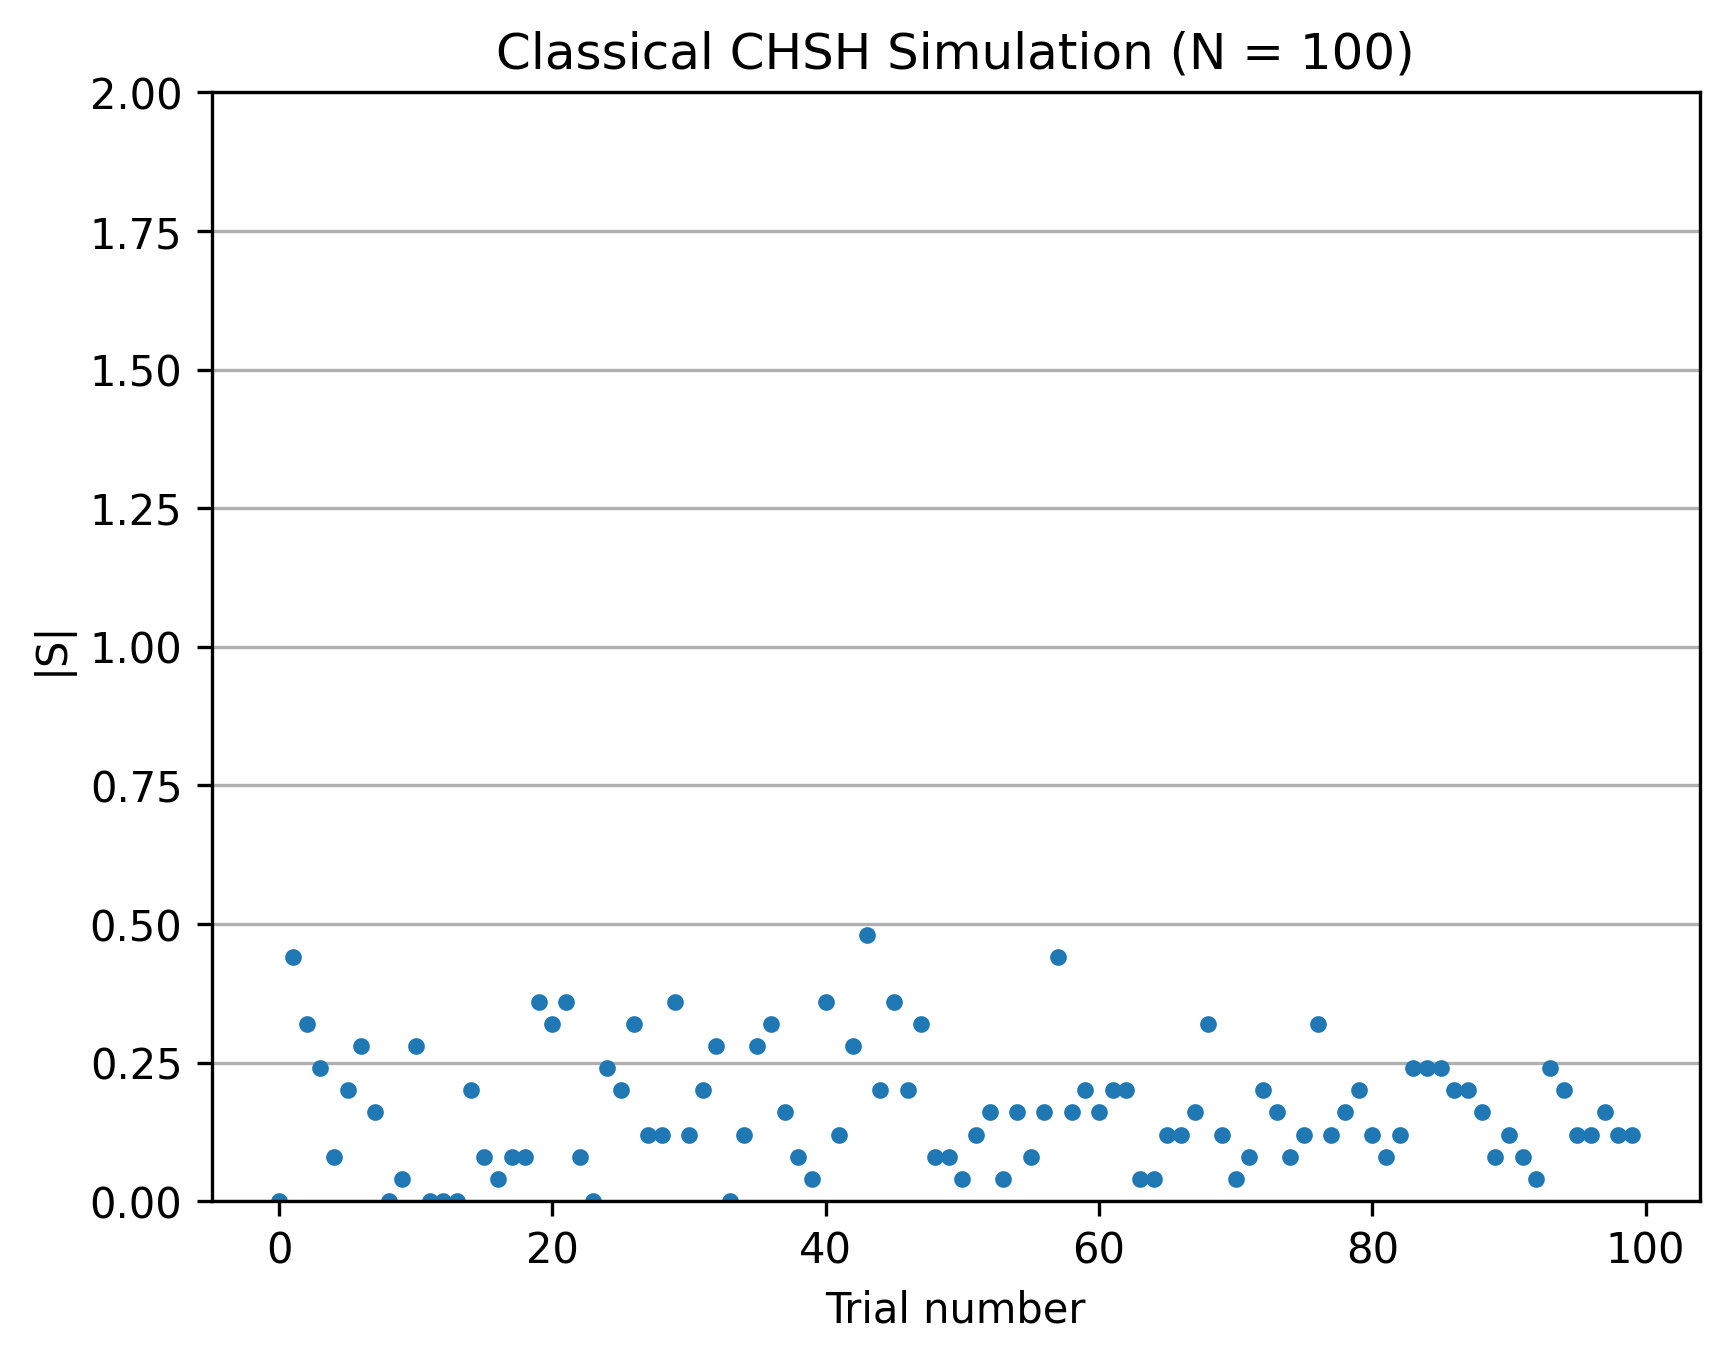
\includegraphics[width=\linewidth]{images/classical_sims/Classical_CHSH_N_100.png}
\end{subfigure}

\vspace{0.1cm}

% ---- Row 4 ----
\begin{subfigure}{0.44\textwidth}
    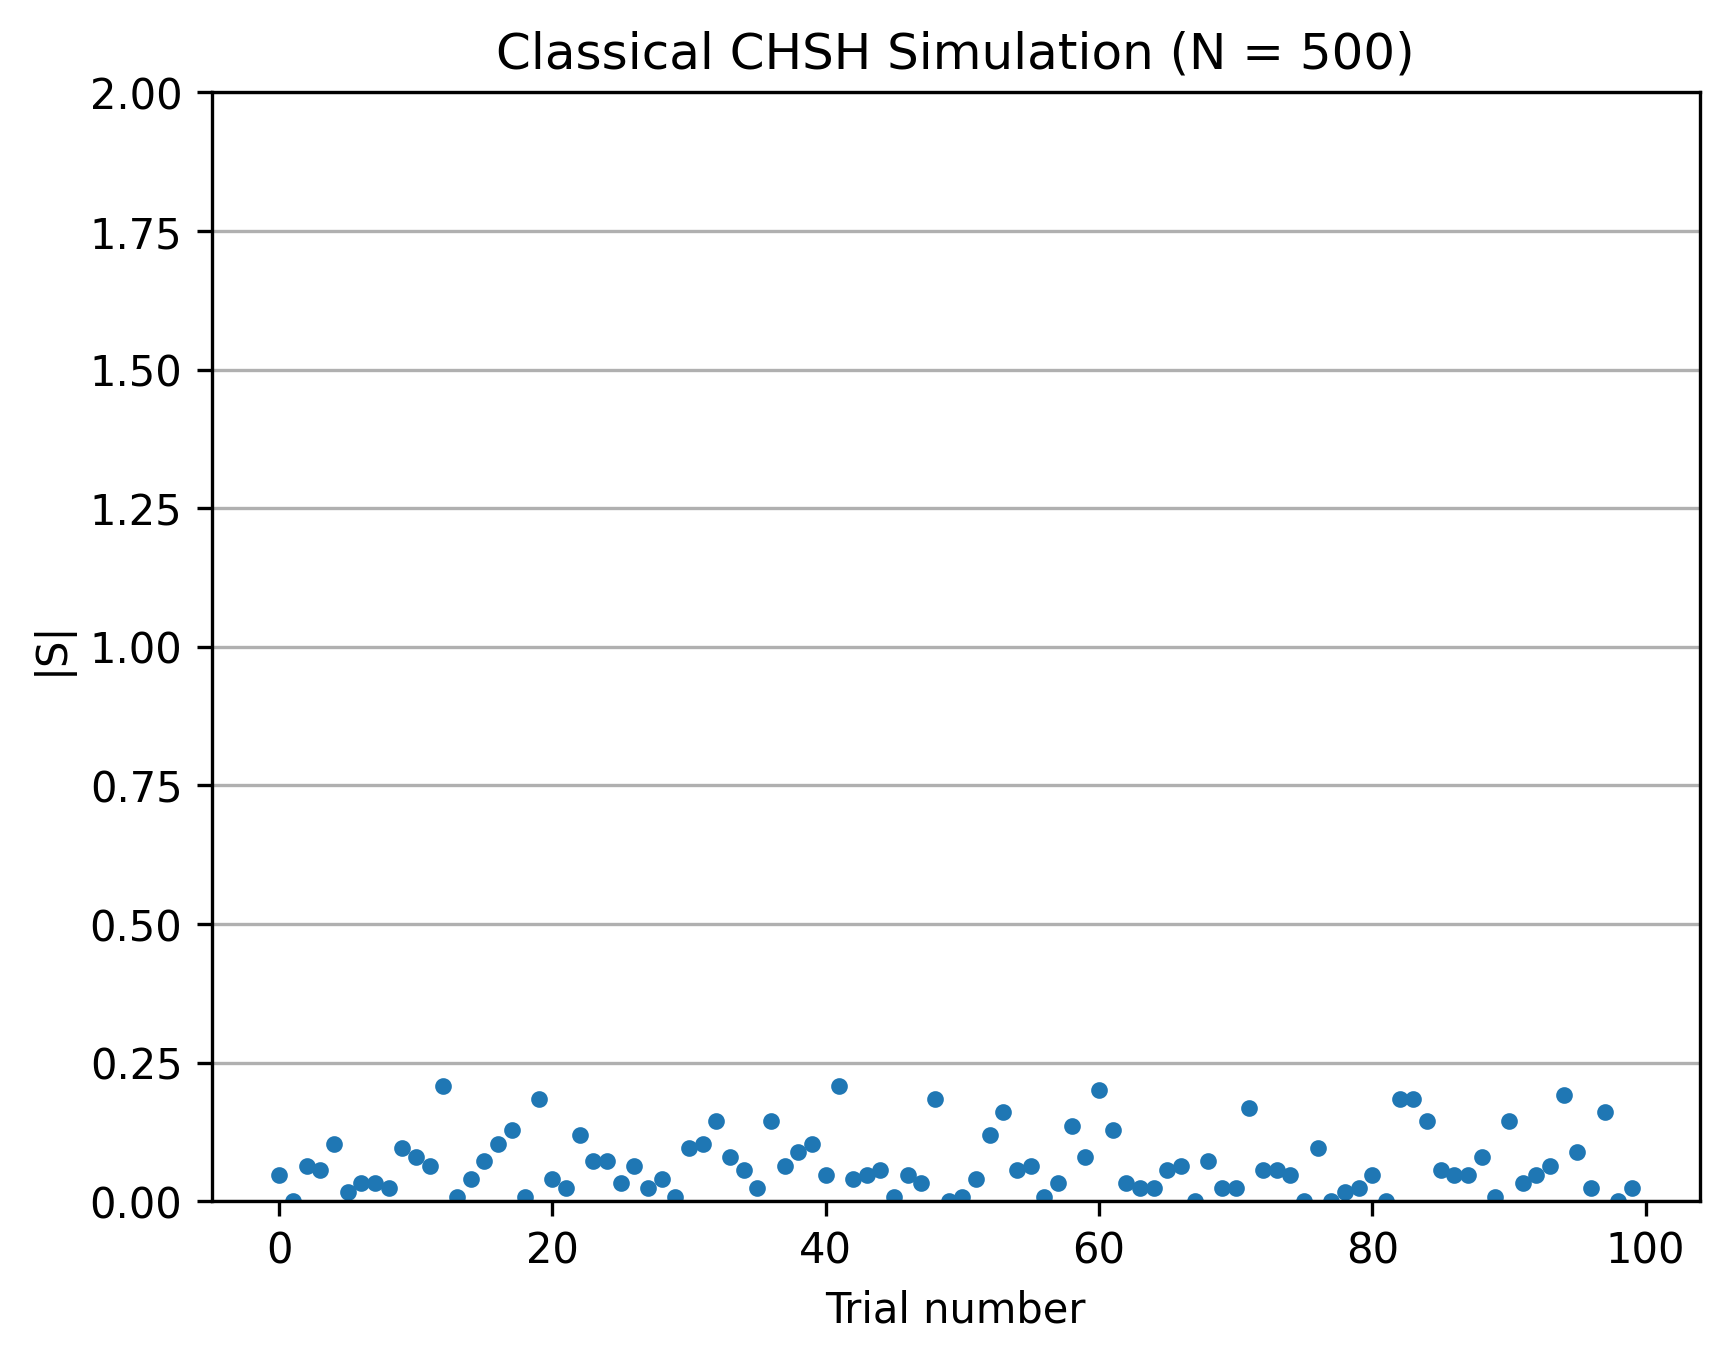
\includegraphics[width=\linewidth]{images/classical_sims/Classical_CHSH_N_500.png}
\end{subfigure}
\hfill
\begin{subfigure}{0.44\textwidth}
    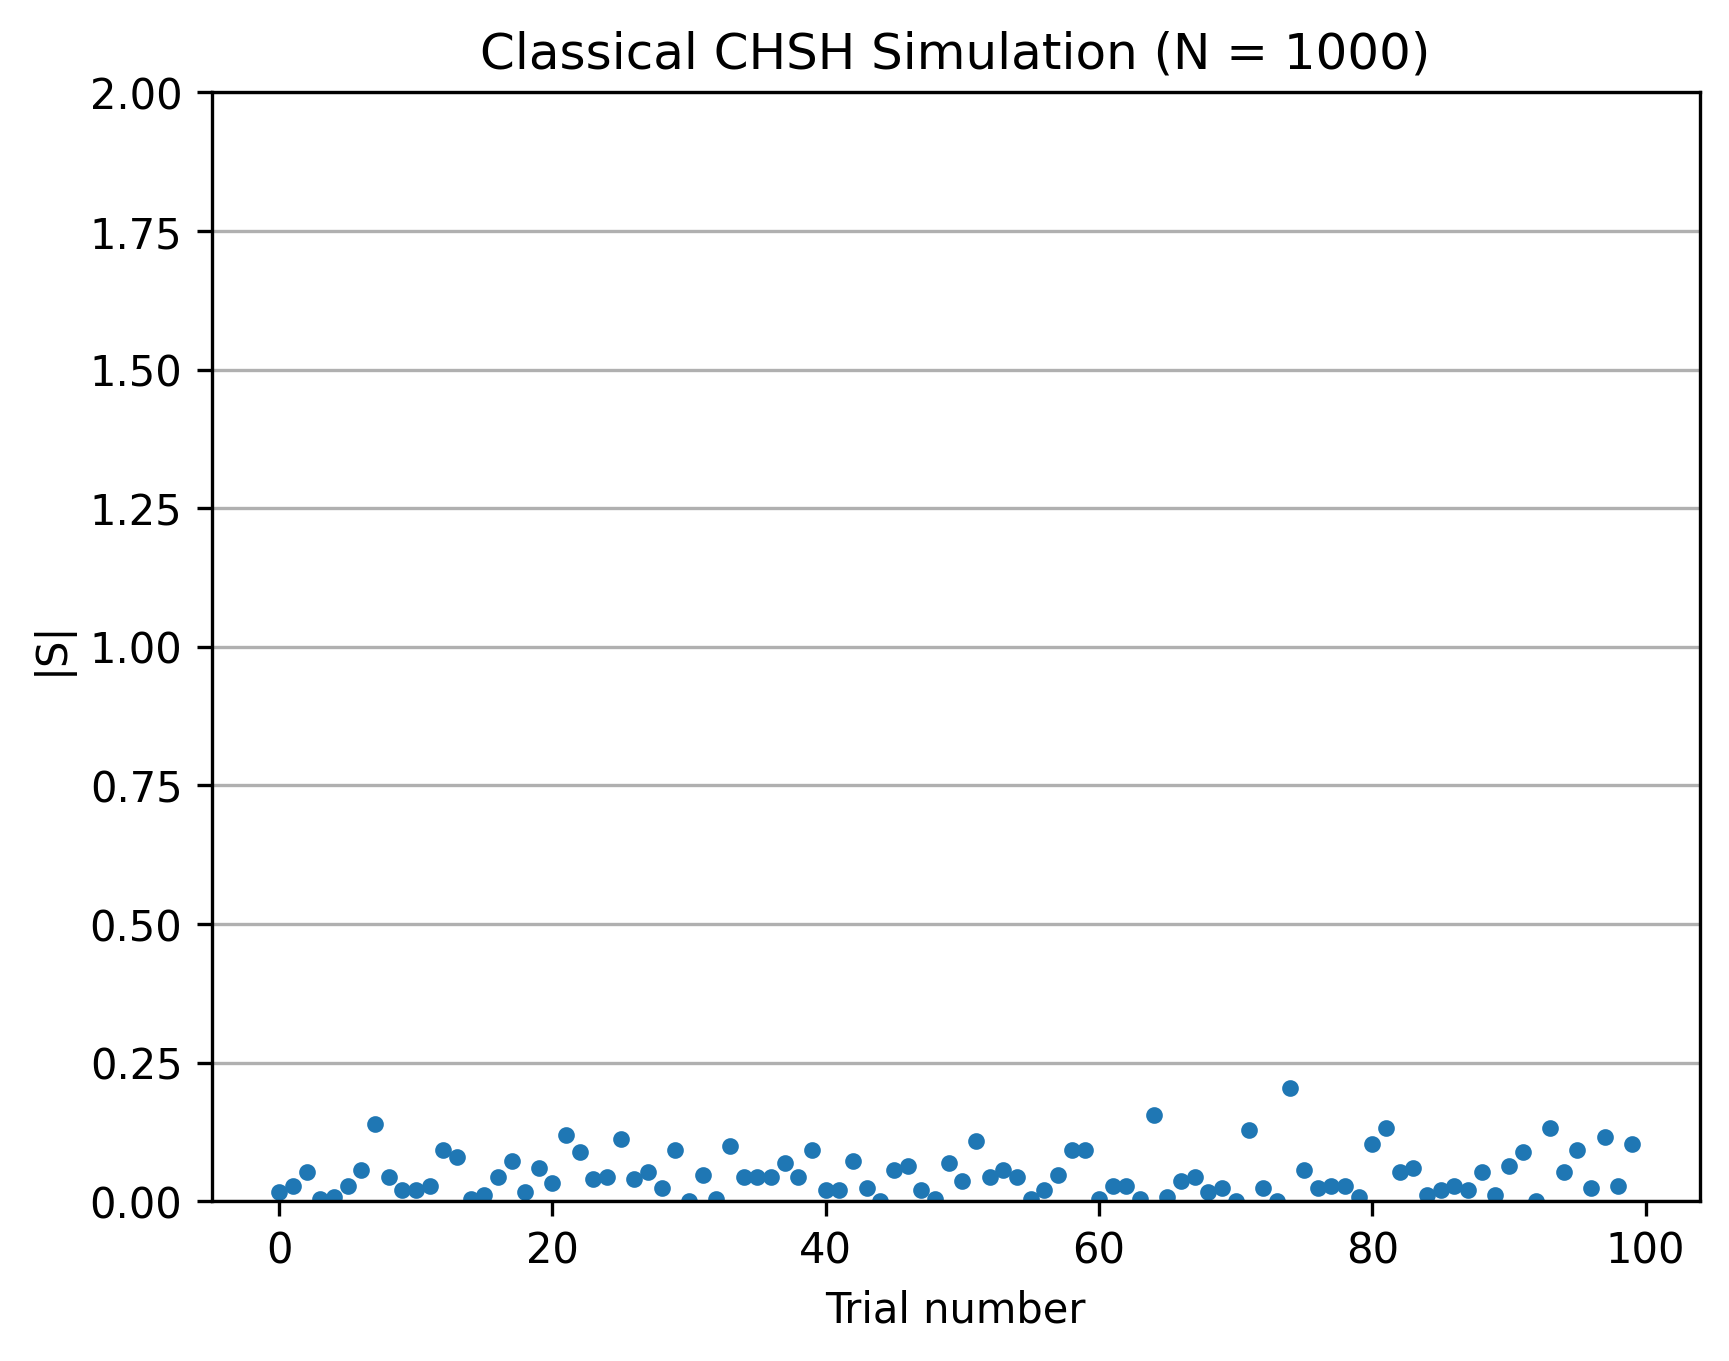
\includegraphics[width=\linewidth]{images/classical_sims/Classical_CHSH_N_1000.png}
\end{subfigure}
\end{figure}
Let's analyze the obtained results
\begin{itemize}
    \item For very small $N$($N$=1,2,4), Each correlation is the average of few $\pm1$ products. So $E_{XX}$,$E_{XY}$,$E_{YX}$,$E_{YY}$ can be $\pm1$ or $\pm0.5$. When calculating CHSH parameter, we get large accidental values. That's why the plots look jumpy.
    \item For moderate $N$($N$=10,50,100), as $N$ increases, random $+1$ and $-1$ outcomes starts start cancelling out and CHSH parameter seems approaching to zero.
    \item For large $N$($N$=500,1000), all correlations $\approx 0$. $|S|$ is very small. Almost all points lie near the bottom.
\end{itemize}
On analyzing the results, we can say, as the number of particle pairs $N$ increases, the value of $|S|$ approaches zero due to statistical averaging in an uncorrelated system. In this simulation, Alice’s and Bob’s outcomes are generated independently, so there is no real correlation between them as there's no shared variable or connection between them. Because of this independence, knowing Alice’s outcome gives no information about Bob’s outcome, and the average product of their results tends to zero.

The above python code is slightly modified to calculate the CHSH parameter of particle pairs $N$ ranging 1-10000 using a nested \textit{for} loop. The CHSH parameter is calculated 10 times for every $N$ and appends to a list. By using \texttt{max()} function the highest value of $|S|$ is appended to another list for plotting the curve. Then a single graph is plotted with $N$ in the x-axis and $|S|$ in the y-axis.
\begin{lstlisting}[language=Python, basicstyle=\ttfamily\footnotesize]
import numpy as np
import matplotlib.pyplot as plt

N = []
S_values = []
S_temp_values = []


def correlation(a, b):
    return np.mean(a * b)


for i in range(10001):
    S_temp_values.clear()
    for j in range(10):
        alice_X = np.random.choice([1, -1], i)
        alice_Y = np.random.choice([1, -1], i)

        bob_X   = np.random.choice([1, -1], i)
        bob_Y   = np.random.choice([1, -1], i)

        E_xx = correlation(alice_X, bob_X)
        E_xy = correlation(alice_X, bob_Y)
        E_yx = correlation(alice_Y, bob_X)
        E_yy = correlation(alice_Y, bob_Y)

        S = E_xx + E_xy + E_yx - E_yy

        S_temp_values.append(abs(S))
    N.append(i)
    S_values.append(np.max(S_temp_values))

plt.plot(N, S_values, ".")

plt.xlabel("N")
plt.ylabel("|S|")
plt.grid(axis="y")
plt.ylim(0, 2)

plt.title(f"Classical CHSH Simulation (N=1-10000)")

plt.savefig(f"Classical_CHSH_N_1-10000.png", dpi=300, bbox_inches="tight")
plt.close()
\end{lstlisting}
\begin{figure}[h]
    \centering
    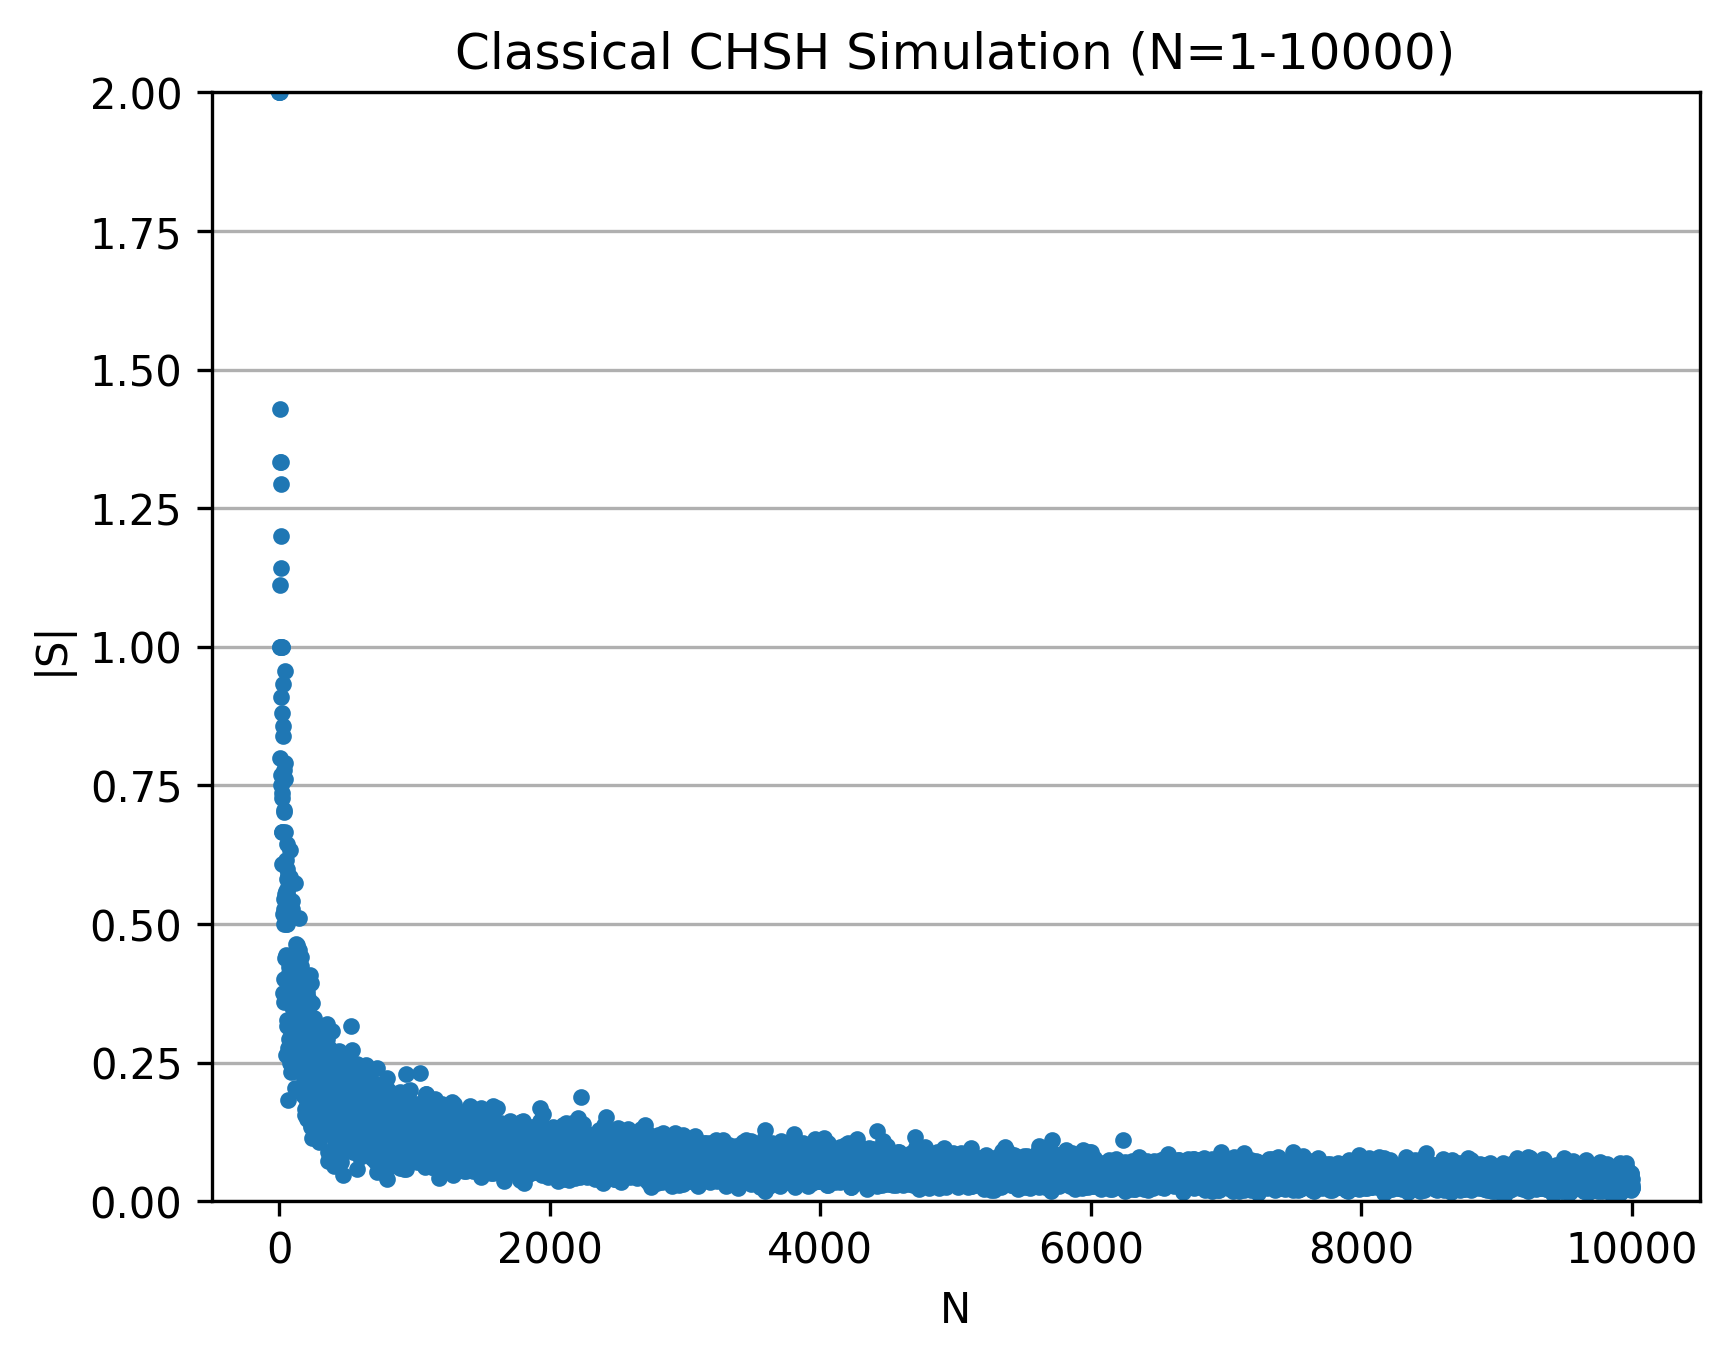
\includegraphics[width=1\textwidth]{images/Classical_CHSH_N_1-10000.png}
\end{figure}
This graph once again confirms that as the number of particle pairs $|S|$ increases, the value of $|S|$ approaches zero due to this uncorrelated system.

By modifying the python code a little bit, we can simulate a correlated system with a \textbf{shared hidden variabe}. In this simulation we are taking $N$ particle pairs and calculating CHSH parameter 1000 times.

Assume Victor secrelty assigns predefined instructions to each particle pairs. For each particle pair, Victor picks a $\lambda$, $\lambda \in \{+1, -1\}$. This is the \textbf{shared hidden variabe}. Now Victor determines what will happen if Alice and Bob mesures the particles. $A_X=\lambda, A_Y=\lambda, B_X=\lambda, B_Y=-\lambda$. This means

\begin{itemize}
\item If Alice measures X $\rightarrow$ she gets $\lambda$, If Alice measures Y $\rightarrow$ she gets $\lambda$
\item If Bob measures X $\rightarrow$ he gets $\lambda$, If Bob measures Y $\rightarrow$ he gets $-\lambda$
\end{itemize}

If $\lambda = -1$, then $A_X=-1, A_Y=-1, B_X=-1$ and $B_Y=+1$.
When we calculate CHSH parameter $S$,
\setcounter{equation}{0}
\begin{equation}
S=E_{XX}+E_{XY}+E_{YX}-E_{YY}
\end{equation}
\begin{equation}
S=(-1 \times -1)+(-1 \times +1)+(-1 \times -1)-(-1 \times +1)
\end{equation}
\begin{equation}
S=1+(-1)+1-(-1)=2
\end{equation}

Now the simulation will give CHSH parameter $|S|=2$, the classical bound for any large no. of particle pairs $N$.

\begin{enumerate}

\item Import NumPy and Matplotlib, Input no. of particle pairs $N$, Define a variabe \texttt{trials = 1000}, Initialize a list \texttt{S\_values} to store calculated CHSH parameter values.
\begin{lstlisting}
import numpy as np
import matplotlib.pyplot as plt

N = int(input("Number of particle pairs per trial: "))
trials = 1000
S_values = []
\end{lstlisting}

\item Define correlation function.
\begin{lstlisting}
def correlation(a, b):
    return np.mean(a * b)
\end{lstlisting}

\item Define correlation function.
\begin{lstlisting}
def correlation(a, b):
    return np.mean(a * b)
\end{lstlisting}

\item Define a \textit{for} loop running \texttt{trials} times. Inside the loop, for every trial, pick $\lambda \in \{+1, -1\}$, then determine measurement outcomes $A_X=\lambda, A_Y=\lambda, B_X=\lambda$ and $B_Y=-\lambda$, calculate correlations, calculate CHSH parameter and append it to list \texttt{S\_values}.
\begin{lstlisting}
for t in range(trials):
    lam = np.random.choice([1, -1], N)

    alice_X = lam
    alice_Y = lam

    bob_X = lam
    bob_Y = -lam

    E_xx = correlation(alice_X, bob_X)
    E_xy = correlation(alice_X, bob_Y)
    E_yx = correlation(alice_Y, bob_X)
    E_yy = correlation(alice_Y, bob_Y)

    S = E_xx + E_xy + E_yx - E_yy
    S_values.append(S)
\end{lstlisting}

\item Then plot curve with trial number in x-axis and $|S|$ in y-axis and save it in PNG format.
\begin{lstlisting}
plt.plot(range(trials), np.abs(S_values), ".")
plt.ylim(0, 3)
plt.xlabel("Trial number")
plt.ylabel("|S|")
plt.title(f"Classical CHSH Simulation (Hidden Variables, N = {N})")
plt.grid(axis="y")
plt.savefig(f"classical_CHSH_hidden_variable_N_{N}.png", dpi=300, bbox_inches="tight")
plt.close()
\end{lstlisting}
\end{enumerate}
\begin{lstlisting}[language=Python, basicstyle=\ttfamily\footnotesize]
import numpy as np
import matplotlib.pyplot as plt

N = int(input("Number of particle pairs per trial: "))
trials = 1000
S_values = []

def correlation(a, b):
    return np.mean(a * b)

for t in range(trials):
    lam = np.random.choice([1, -1], N)

    alice_X = lam
    alice_Y = lam

    bob_X = lam
    bob_Y = -lam

    E_xx = correlation(alice_X, bob_X)
    E_xy = correlation(alice_X, bob_Y)
    E_yx = correlation(alice_Y, bob_X)
    E_yy = correlation(alice_Y, bob_Y)

    S = E_xx + E_xy + E_yx - E_yy
    S_values.append(S)

plt.plot(range(trials), np.abs(S_values), ".")
plt.ylim(0, 3)
plt.xlabel("Trial number")
plt.ylabel("|S|")
plt.title(f"Classical CHSH Simulation (Hidden Variables, N = {N})")
plt.grid(axis="y")
plt.savefig(f"classical_CHSH_hidden_variable_N_{N}.png", dpi=300, bbox_inches="tight")
plt.close()

\end{lstlisting}
\begin{figure}[H]
    \centering
    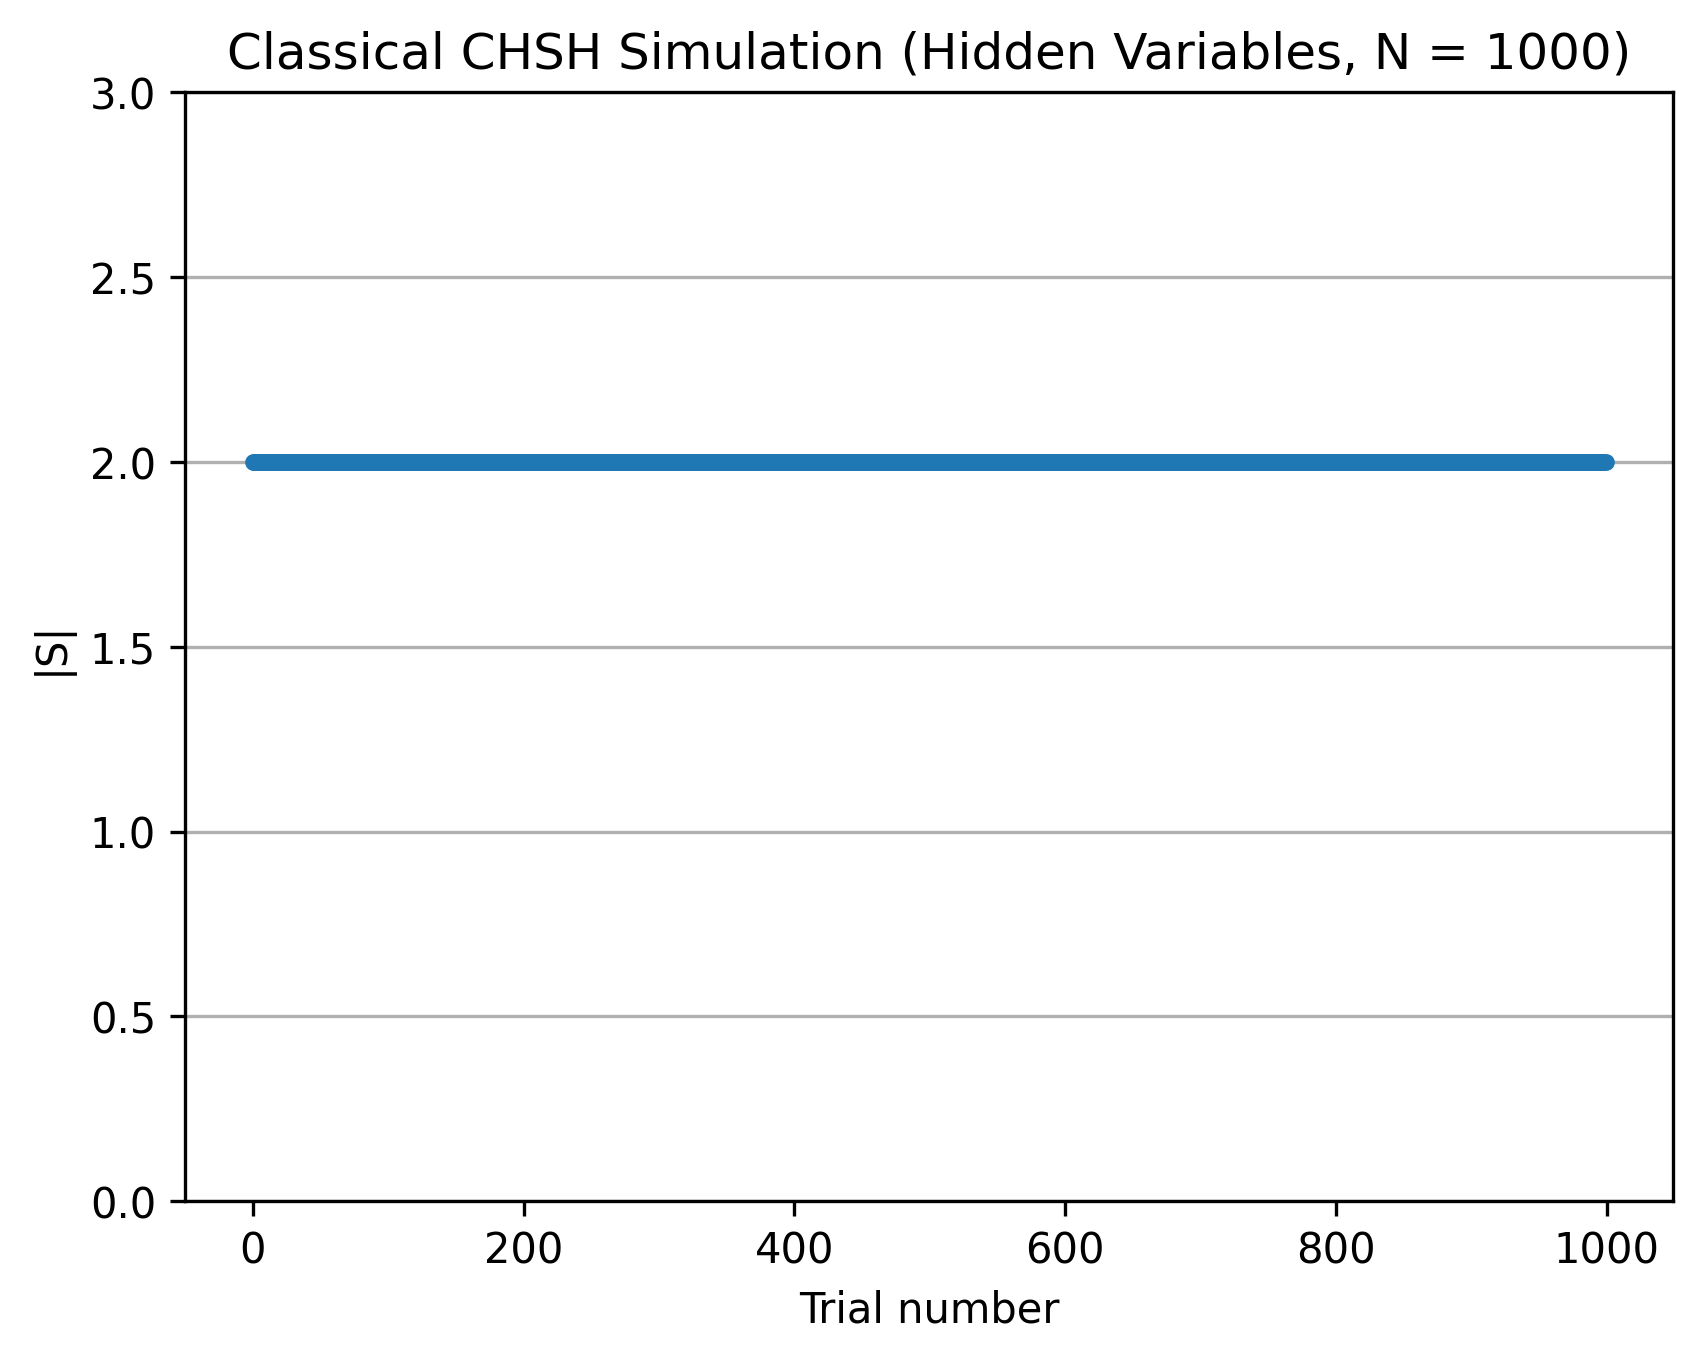
\includegraphics[width=1\textwidth]{images/classical_CHSH_hidden_variable_N_1000.png}
\end{figure}

The classical CHSH simulation based on a local hidden-variable (LHV) demonstrates that correlations between particle pairs can be fully explained by predetermined instructions given at the source. In this model, each particle pair carries a hidden variable that fixes the outcomes of all possible measurements before Alice and Bob perform them. By computing the correlation functions over many trials and evaluating the CHSH parameter, it is observed that the value of $|S|$ never exceeds the classical bound of 2. This confirms Bell’s result that no classical local hidden-variable theory can reproduce the stronger correlations predicted by quantum mechanics.

\subsection*{Quantum Mechanical Predictions}

Quantum mechanics predicts correlations between entangled particles are stronger than those allowed by classical physics. When a pair of particles is prepared in an entangled state, the measurement outcomes obtained by Alice and Bob are not independent, even when the particles are separated by large distances. These quantum correlations depend on the choice of measurement settings.

For the CHSH experiment, quantum mechanics predicts specific values for the correlation functions based on the quantum state and the measurement directions chosen by the observers. When these quantum correlations are combined to calculate the CHSH parameter $S$, the result can exceed the classical limit of 2. The maximum value predicted by quantum mechanics is $2\sqrt{2}$. This upper limit is known as \textbf{Tsirelson’s bound}.

Let's try to understand how the quantum upper limit became $2\sqrt{2}$. Starts with a \textbf{Singlet State}. A singlet state is a quantum entangled state of two spin-1/2 particles (like two electrons) with total spin zero, described by the wavefunction $\frac{1}{\sqrt{2}}\left(\lvert \uparrow \downarrow \rangle - \lvert \downarrow \uparrow \rangle\right)$. In our case, $\frac{1}{\sqrt{2}}\left(\lvert 01 \rangle - \lvert 10 \rangle\right)$. This means
\begin{itemize}
\item $\lvert 0 \rangle \rightarrow$ spin up
\item $\lvert 1 \rangle \rightarrow$ spin down
\end{itemize}
For two particles:
\begin{itemize}
\item $\lvert 01 \rangle \rightarrow$ Alice = up, Bob = down
\item $\lvert 10 \rangle \rightarrow$ Alice = down, Bob = up
\end{itemize}
The system is in a superposition of (Alice up, Bob down) and (Alice down, Bob up).

If Alice and Bob measure spin along directions \textbf{a} and \textbf{b}, then measurement along direction \textbf{a} is represented by operator $A = \vec{a} \cdot \vec{\sigma}$. Similarly for \textbf{b}: $B = \vec{b} \cdot \vec{\sigma}$. Here $\vec{\sigma} = (\sigma_x, \sigma_y, \sigma_z)$. These are \textbf{Pauli matrices}. $\vec{a}$ and $\vec{b}$ are unit vectors. So the measurement results are $\pm1$.

Quantum mathematically, correlation means
\setcounter{equation}{0}
\begin{equation}
E(a,b) = \langle \psi^- \mid (\vec{a} \cdot \vec{\sigma}) \otimes (\vec{b} \cdot \vec{\sigma}) \mid \psi^- \rangle
\end{equation}
Expand $(\vec{a} \cdot \vec{\sigma}) \otimes (\vec{b} \cdot \vec{\sigma})$,
The dot products:
\[
\begin{aligned}
\vec{a} \cdot \vec{\sigma} &= a_x \sigma_x + a_y \sigma_y + a_z \sigma_z \\
\vec{b} \cdot \vec{\sigma} &= b_x \sigma_x + b_y \sigma_y + b_z \sigma_z
\end{aligned}
\]
The expansion becomes:
\begin{equation}
E(a,b)=(a_x \sigma_x + a_y \sigma_y + a_z \sigma_z)
\otimes
(b_x \sigma_x + b_y \sigma_y + b_z \sigma_z)
\end{equation}
Use distributice rule:
\[
(A + B) \otimes (C + D) = A \otimes C + A \otimes D + B \otimes C + B \otimes D
\]

\begin{equation}
\begin{aligned}
E(a,b)&= a_x b_x (\sigma_x \otimes \sigma_x) + a_x b_y (\sigma_x \otimes \sigma_y) + a_x b_z (\sigma_x \otimes \sigma_z) \\
&\quad + a_y b_x (\sigma_y \otimes \sigma_x) + a_y b_y (\sigma_y \otimes \sigma_y) + a_y b_z (\sigma_y \otimes \sigma_z) \\
&\quad + a_z b_x (\sigma_z \otimes \sigma_x) + a_z b_y (\sigma_z \otimes \sigma_y) + a_z b_z (\sigma_z \otimes \sigma_z)
\end{aligned}
\end{equation}
We can write it in a compact form:
\begin{equation}
E(a,b) = \sum_{i,j} a_i b_j \, \langle \sigma_i \otimes \sigma_j \rangle
\end{equation}
Since the total spin equals zero, the quantum state shows perfect rotational symmetry and anti-correlation in all direction. If Alice and Bob measure spin along the same axis, the measurement are perfectly anti-correlated($-1$). If they measure along different axes, there is no correlation($0$).
\[
\langle \sigma_i \otimes \sigma_j \rangle = -\delta_{ij}
\]
\[
\delta_{ij} =
\begin{cases}
1 & i = j \\
0 & i \ne j
\end{cases}
\]

\begin{itemize}
\item If $i=j$, $\langle \sigma_i \otimes \sigma_j \rangle=-1$
\item If $i \neq j$, $\langle \sigma_i \otimes \sigma_j \rangle=0$
\end{itemize}

Only terms where $i=j$ survive.
\begin{equation}
E(a,b) = - \sum_i a_i b_i
\end{equation}
That sum is exactly the dot product.
\begin{equation}
E(a,b) = - \vec{a} \cdot \vec{b}
\end{equation}
For unit vectors, $\vec{a} \cdot \vec{b} = \cos \theta$. And the correlation becomes
\begin{equation}
E(a,b) = - \cos \theta
\end{equation}
$\theta$ is the angle between measurement directions.

Now we got the equation for calculation correlation. We know quantum mechanics violates CHSH inequality, to get the maximum violation, we choose special measurement angles.
\begin{itemize}
\item $a=0^\circ$
\item $a'=90^\circ$
\item $b=45^\circ$
\item $b'=-45^\circ$
\end{itemize}
Calculating the CHSH parameter,
\[
S = E(a,b) + E(a,b') + E(a',b) - E(a',b')
\]
Substituting the values,
\[
S = E(45^\circ,0^\circ) + E(0^\circ,-45^\circ) + E(90^\circ,45^\circ) - E(90^\circ,-45^\circ)
\]
\begin{equation*}
\begin{aligned}
S &= (-\cos(45^\circ-0^\circ)) + (-\cos(0^\circ--45^\circ)) \\
&\quad+ (-\cos((90^\circ-45^\circ)) - (-\cos(90^\circ--45^\circ))
\end{aligned}
\end{equation*}
\[
S = (-\cos(45^\circ)) + (-\cos(45^\circ)) + (-\cos((45^\circ)) - (-\cos((135^\circ))
\]
\[
S = -\frac{\sqrt{2}}{2} - \frac{\sqrt{2}}{2} - \frac{\sqrt{2}}{2} - \frac{\sqrt{2}}{2}
\]
\[
S = -2\sqrt{2}
\]
\[
|S| = 2\sqrt{2} \approx 2.8284
\]
For a quantum mechanical system the CHSH parameter $|S| \leq 2\sqrt{2}$, which is greater than the classical limit of 2. This is the clear violation of CHSH inequality. This result serves as a strong evidence for the existance of quantum effects in nature.

\subsubsection*{Python Simulation}
\begin{enumerate}
\item Import NumPy module, define no. of particle pairs $N=100000$ and define measurement angles in radian.
\begin{lstlisting}
import numpy as np

N = 100000

a  = 0
a_p = np.pi/2
b  = np.pi/4
b_p = -np.pi/4
\end{lstlisting}
\item Define a function to calculate quantum correlation which takes a parameter \texttt{theta} which is the  angle between measurement directions. Every time this function is called, it creates a local variable \texttt{p\_same} which is the probability of measured outcome is the same.

Let's understand how it is calculated, The correlation is defined as $E = \langle A \times B \rangle$. $A$ and $B$ have outcome $\pm1$. If
\begin{itemize}
\item outcomes are the same $\rightarrow$ product = $+1$
\item outcomes are different $\rightarrow$ product = $-1$
\end{itemize}
Let:
\begin{itemize}
\item $P(same)=$ probability that $A$ and $B$ are equal
\item $P(different)=$ probability that $A$ and $B$ are opposite
\end{itemize}
Since those are thy only two possibilities:
{
\renewcommand{\theequation}{\Alph{equation}}
\setcounter{equation}{0}
\begin{equation}
P(same)+P(different)=1
\end{equation}
}
Now calculate the average $E$:
\setcounter{equation}{0}
\begin{equation}
E=(+1) \times P(same) + (-1) \times P(different)
\end{equation}
\begin{equation}
E=P(same) - P(different)
\end{equation}
We know that for a singlet state $E = - \cos \theta$
{
\renewcommand{\theequation}{\Alph{equation}}
\setcounter{equation}{1}
\begin{equation}
P(same) - P(different) = - \cos \theta
\end{equation}
}
Add equation $(A)$ and $(B)$
\setcounter{equation}{0}
\begin{equation}
2 \times P(same) = 1 - \cos \theta
\end{equation}
\begin{equation}
P(\text{same}) = \frac{1 - \cos \theta}{2}
\end{equation}
Inside the function, add a list \texttt{results} to store correlation values. Then run a \textit{for} loop $N$ times. In every run, generate a random number less then one, if it is less then \texttt{p\_same}, $A$ and $B$ have same outcome($A=B$). Else, opposite outcome($A=-B$) then append correlation value($A \times B$) to \texttt{results}. After the loop is completed, return the mean of \texttt{results}.
\begin{lstlisting}
def quantum_correlation(theta):
    p_same = (1 - np.cos(theta)) / 2
    results = []
    for _ in range(N):
        if np.random.rand() < p_same:
            A = np.random.choice([1, -1])
            B = A
        else:
            A = np.random.choice([1, -1])
            B = -A

        results.append(A * B)
    return np.mean(results)
\end{lstlisting}
\item Compute all four correlations by calling the above function and calculate $S$ then print all results.
\begin{lstlisting}
E_ab   = quantum_correlation(a - b)
E_ab_p = quantum_correlation(a - b_p)
E_a_p_b = quantum_correlation(a_p - b)
E_a_p_b_p = quantum_correlation(a_p - b_p)

S = E_ab + E_ab_p + E_a_p_b - E_a_p_b_p

print("E(a,b)      =", E_ab)
print("E(a,b')     =", E_ab_p)
print("E(a',b)     =", E_a_p_b)
print("E(a',b')    =", E_a_p_b_p)
print("\nCHSH S =", S)
print("|S| =", abs(S))
\end{lstlisting}
\end{enumerate}
\begin{lstlisting}[language=Python, basicstyle=\ttfamily\footnotesize]
import numpy as np

N = 100000

a  = 0
a_p = np.pi/2
b  = np.pi/4
b_p = -np.pi/4

def quantum_correlation(theta):
    p_same = (1 - np.cos(theta)) / 2
    results = []
    for _ in range(N):
        if np.random.rand() < p_same:
            A = np.random.choice([1, -1])
            B = A
        else:
            A = np.random.choice([1, -1])
            B = -A

        results.append(A * B)
    return np.mean(results)

E_ab   = quantum_correlation(a - b)
E_ab_p = quantum_correlation(a - b_p)
E_a_p_b = quantum_correlation(a_p - b)
E_a_p_b_p = quantum_correlation(a_p - b_p)

S = E_ab + E_ab_p + E_a_p_b - E_a_p_b_p

print("E(a,b)      =", E_ab)
print("E(a,b')     =", E_ab_p)
print("E(a',b)     =", E_a_p_b)
print("E(a',b')    =", E_a_p_b_p)
print("\nCHSH S =", S)
print("|S| =", abs(S))
\end{lstlisting}
\subsubsection*{Simulation Result}
\begin{figure}[H]
    \centering
    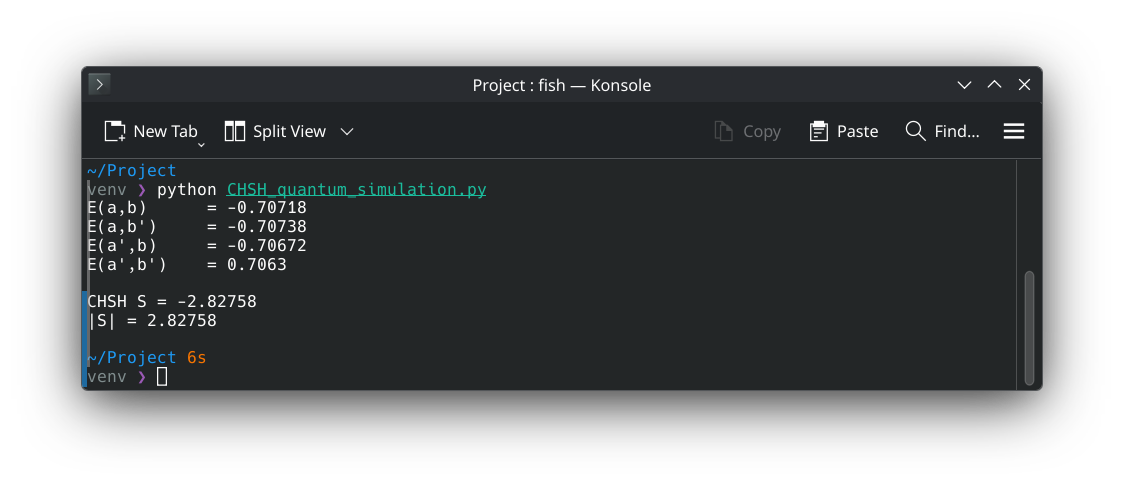
\includegraphics[width=1\textwidth]{images/CHSH_quantum_result.png}
\end{figure}
The obtained simulations value of $|S|$ is $2.82758$. Which is less than the maximum value $2 \sqrt{2} \approx 2.82842$. Since the obtained value is greater than the classical CHSH limit of $2$, it is confirmed that quantum mechanics violates CHSH inequality.

The CHSH inequality plays a role in understanding the difference between classical and quantum physics. Its violation shows that the behavior of entangled particles cannot be explained using classical theories alone. Instead, it reveals that quantum systems exhibit correlations that are unique in nature.


\end{document}
